\subsection{Базовый комплект}\label{ssec:basic-set}

%%%%%%%%%%%%%%%%%%%%%%%%%%%%%%%%%%%%%%%%%%%%%%%%%%%%%%%%%
\subsubsection{Содержание базового комплекта}
%%%%%%%%%%%%%%%%%%%%%%%%%%%%%%%%%%%%%%%%%%%%%%%%%%%%%%%%%

\begin{itemize}[noitemsep]
  \item Для записи видео:
        \begin{itemize}
          \item Камера \textsf{HXR-NX100}.
          \item \textsf{SD} карта памяти (64гб или 128гб, вставлена в камеру).
          \item Аккумулятор для камеры (вставлен в камеру).
          \item Крышка объектива.
          \item Штатив + чехол.
        \end{itemize}
        \vspace{5pt}

  \item Для записи звука:
        \begin{itemize}
          \item Радио-микрофон \textsf{Sennheiser EW 100 ENGG4-A (receiver)}. Также к нему:
                \begin{itemize}
                  \item 2 аккумуляторные батарейки (вставлены в микрофон).
                  \item Петличный микрофон (провод с микрофоном).
                \end{itemize}

          \item Радио-микрофон \textsf{Sennheiser EW 100 ENGG4-A (transmitter)}. Также к нему:
                \begin{itemize}
                  \item 2 аккумуляторные батарейки (вставлены в микрофон).
                  \item Переходник \textsf{XLR -- 3.5 mm jack} (для подключения к камере).
                \end{itemize}
        \end{itemize}
        \vspace{5pt}

  \item Рюкзак для камеры и микрофонов.
        \vspace{5pt}

  \item Опционально по ситуации:
        \begin{itemize}
          \item 4 запасные аккумуляторные батарейки.
          \item Наушник для прослушивания звука с камеры.
          \item Запасной аккумулятор для камеры.
          \item Зарядное от камеры + удлинитель.
        \end{itemize}
\end{itemize}
\vspace{10pt}

%%%%%%%%%%%%%%%%%%%%%%%%%%%%%%%%%%%%%%%%%%%%%%%%%%%%%%%%%
\subsubsection{Описание базового комплекта}
%%%%%%%%%%%%%%%%%%%%%%%%%%%%%%%%%%%%%%%%%%%%%%%%%%%%%%%%%

В базовый комплект входит штатив и чёрный рюкзак с камерой. В рюкзаке есть 2 отделения. В отделении ближе к спине лежит камера, петлички и провода для них. Во втором отделении обычно располагается зарядка от камеры, пирамидка (avermedia) и провода для неё.

\noindent\begin{minipage}[c]{0.45\textwidth}
  \centering
  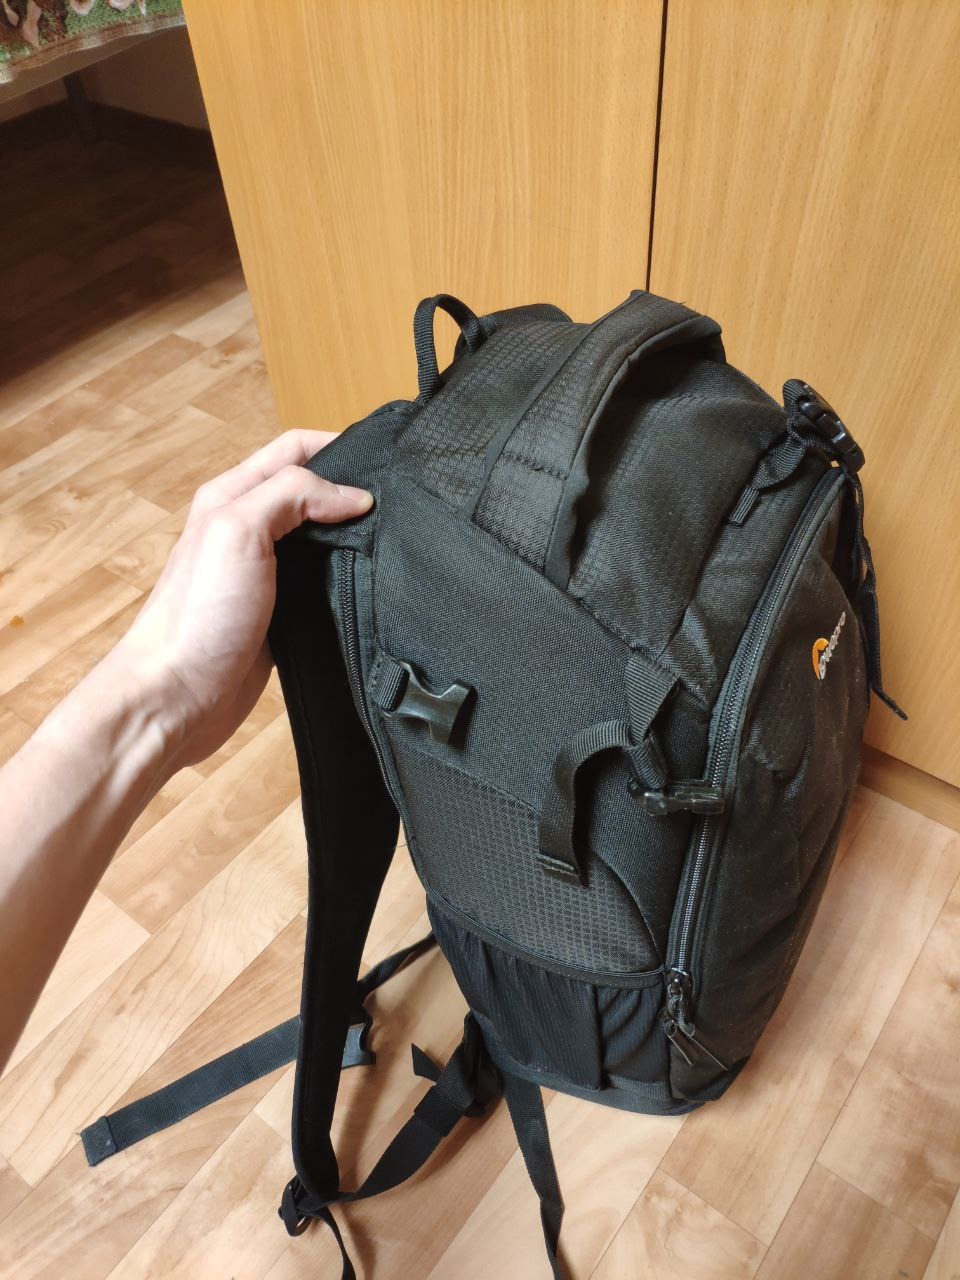
\includegraphics[width=0.6\textwidth]{Images/PortableCamera/BasicSet/bag.jpg}
\end{minipage}
% \hfill
\begin{minipage}[c]{0.45\textwidth}
  \centering
  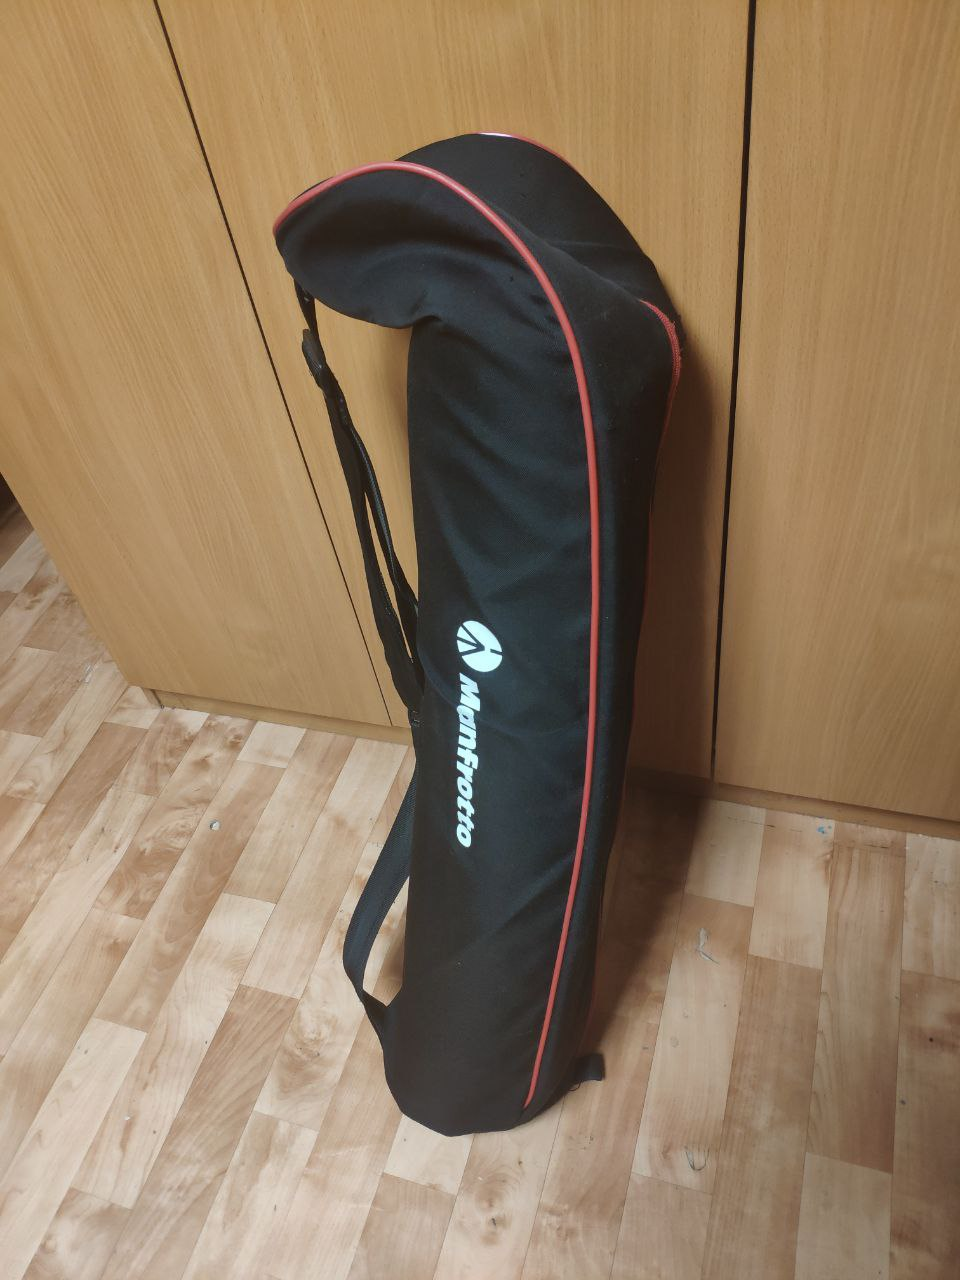
\includegraphics[width=0.6\textwidth]{Images/PortableCamera/BasicSet/tripod.jpg}
\end{minipage}

В отделении с камерой есть 3 кармана:
\begin{itemize}
  \item В верхнем оделении лежит петличный микрофон (провод) и переходник \textsf{XLR -- 3.5 mm jack}. Опцинально здесь может лежать запасной аккумулятор от камеры.

  \item В открытом отделении справа расположены петлички.

  \item В отделении снизу пасполагается наушник (опционально) и запасные аккумы для петличек.
\end{itemize}

\begin{center}
  \begin{minipage}[c]{\textwidth}\label{fig:bag-open}
    \centering
    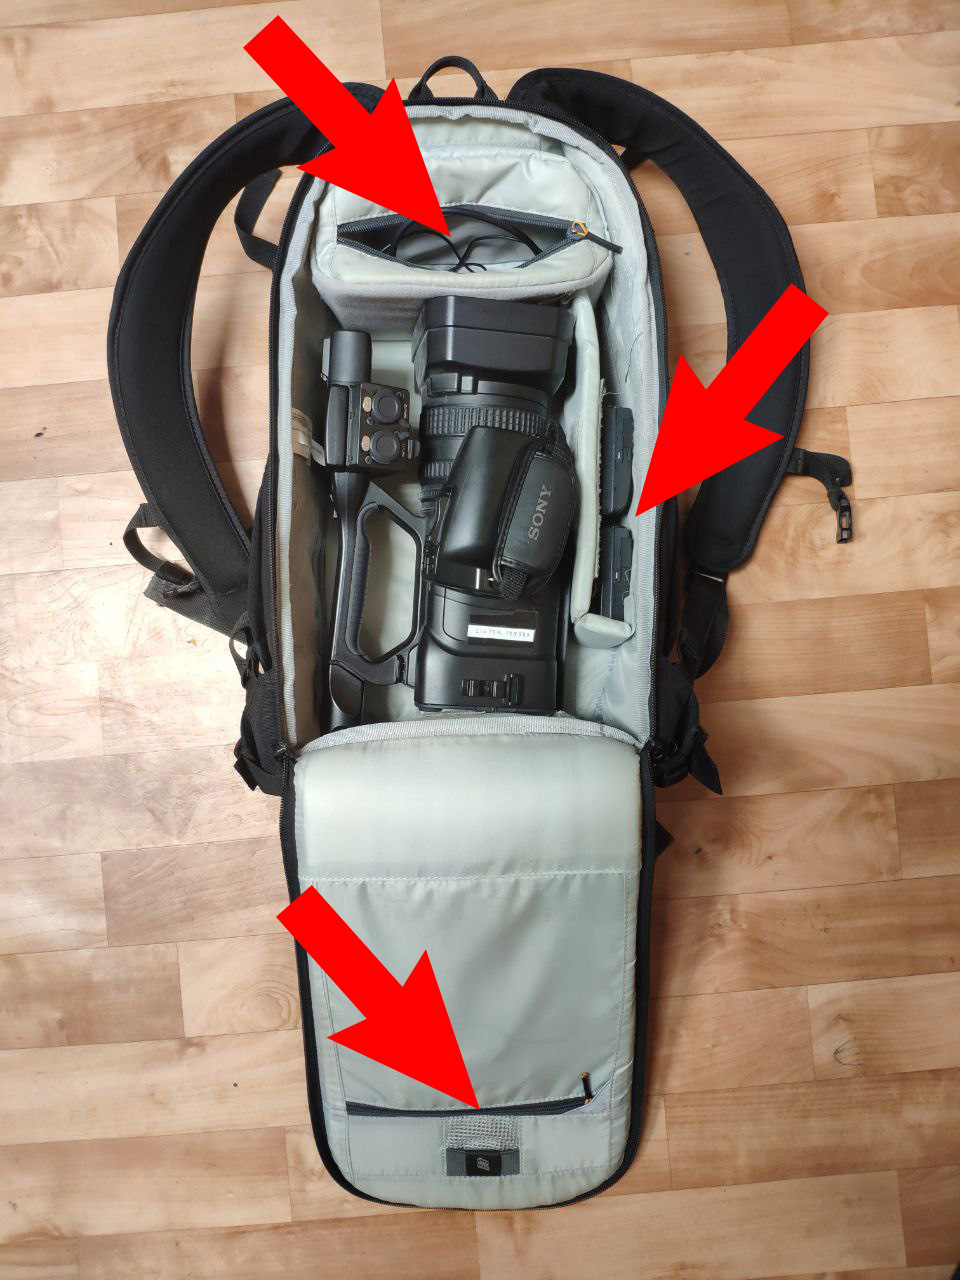
\includegraphics[width=0.4\textwidth]{Images/PortableCamera/BasicSet/bag-open.jpg}
  \end{minipage}
\end{center}

\subsubsection{Как собирать основной комплект}

\begin{tcolorbox}
  При сборке-разборке \textbf{не зажимайте крепежи} слишком сильно. Во-первых, они от этого быстрее изнашиваются, а во-вторых --- на переносную камеру снимают не только парни :) .
\end{tcolorbox}

\begin{enumerate}

  \item Забрать у ответственного \textbf{рюкзак с камерой} $+$ \textbf{штатив} и заранее подойти в аудиторию.

  \item Собрать штатив:
        \begin{enumerate}
          \item Отстегнуть липучку и достать штатив из чехла.

                \par Обратите внимание, как расположен штатив в чехле на картинке --- голова штатива появляется первой после расстёгивания молнии. Аналогично его надо будет складывать обратно.

                \begin{center}
                  \begin{minipage}[c]{0.4\textwidth}
                    \centering
                    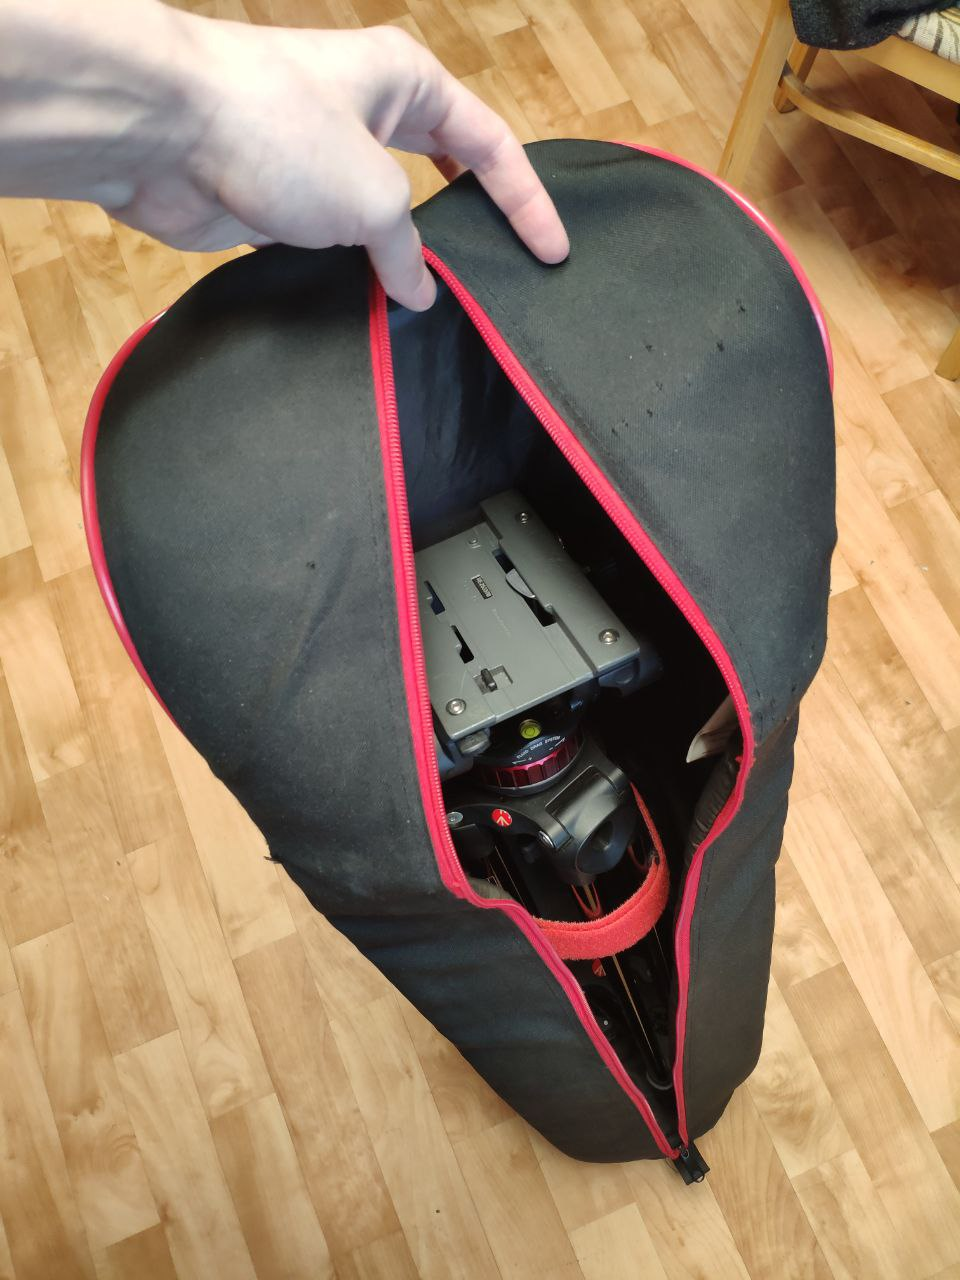
\includegraphics[width=\textwidth]{PortableCamera/tripod/step2.1-in-case.jpg}
                  \end{minipage}
                \end{center}

          \item Установить штатив на нужную высоту.
                \par Поставить штатив в положение на рисунке 2, отстегнуть все серые зажимы и, оставляя ноги на полу, вытянуть штатив на высоту, достаточную для съёмки\footnote{После того, как вы вытянули штатив на нужную высоту, некоторые ножки могли не полностью выйти --- в таком случае нужно вытянуть их самостоятельно}. Затянуть все серые зажимы\footnote{Держитесь за одну из ног штатива, как на фото --- так будет удобнее и он не упадёт.} \textbf{и только после этого}\footnote{Если расставить ноги раньше, то закрепить штатив будет намного сложнее.} расставить ноги (у штатива :) ).

                \begin{minipage}[c]{0.28\textwidth}
                  \centering
                  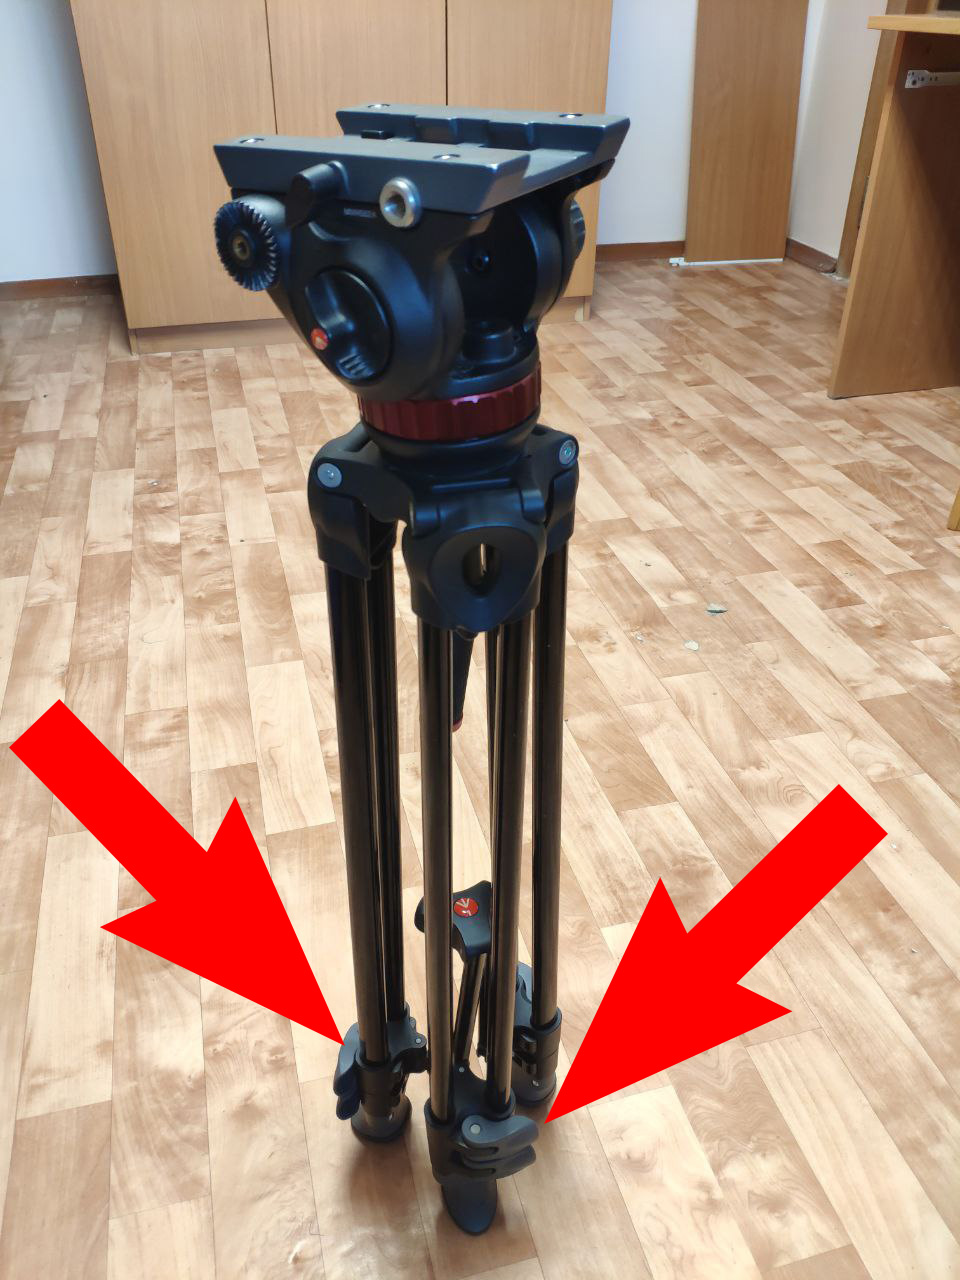
\includegraphics[width=\textwidth]{PortableCamera/tripod/step2.2-1-folded.jpg}
                \end{minipage}
                \hfill
                \begin{minipage}[c]{0.28\textwidth}
                  \centering
                  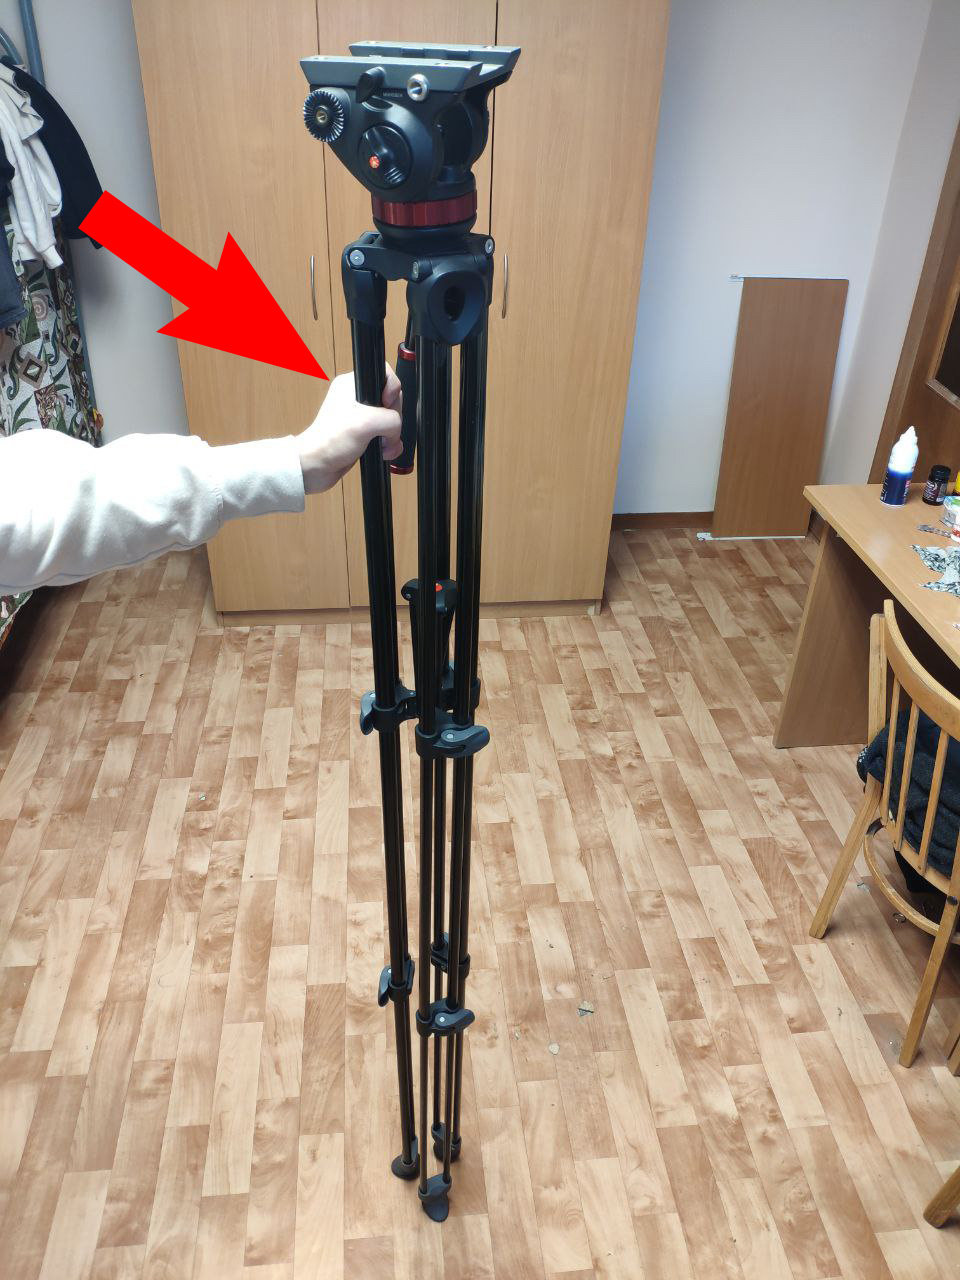
\includegraphics[width=\textwidth]{PortableCamera/tripod/step2.2-2-height.jpg}
                \end{minipage}
                \hfill
                \begin{minipage}[c]{0.28\textwidth}
                  \centering
                  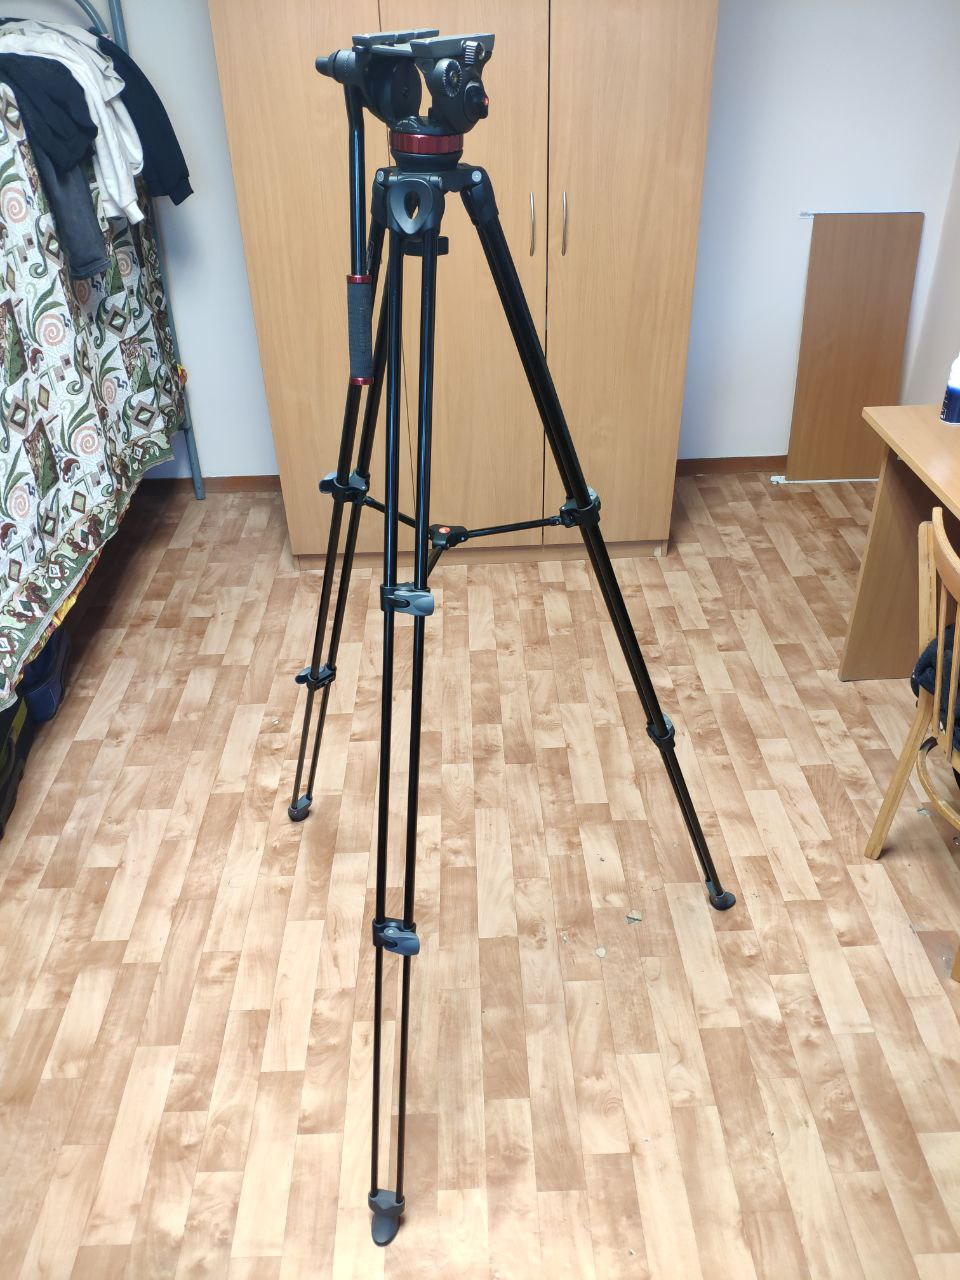
\includegraphics[width=\textwidth]{PortableCamera/tripod/step2.2-3-legs-apart.jpg}
                \end{minipage}

          \item Зафиксировать ручку в удобном положении.
                \par Для этого открутить её крепёж (против часовой стрелки), пока не разойдутся зубчики, повернуть её в удобное положение и закрутить крепёж обратно.

                \begin{minipage}[c]{0.43\textwidth}
                  \centering
                  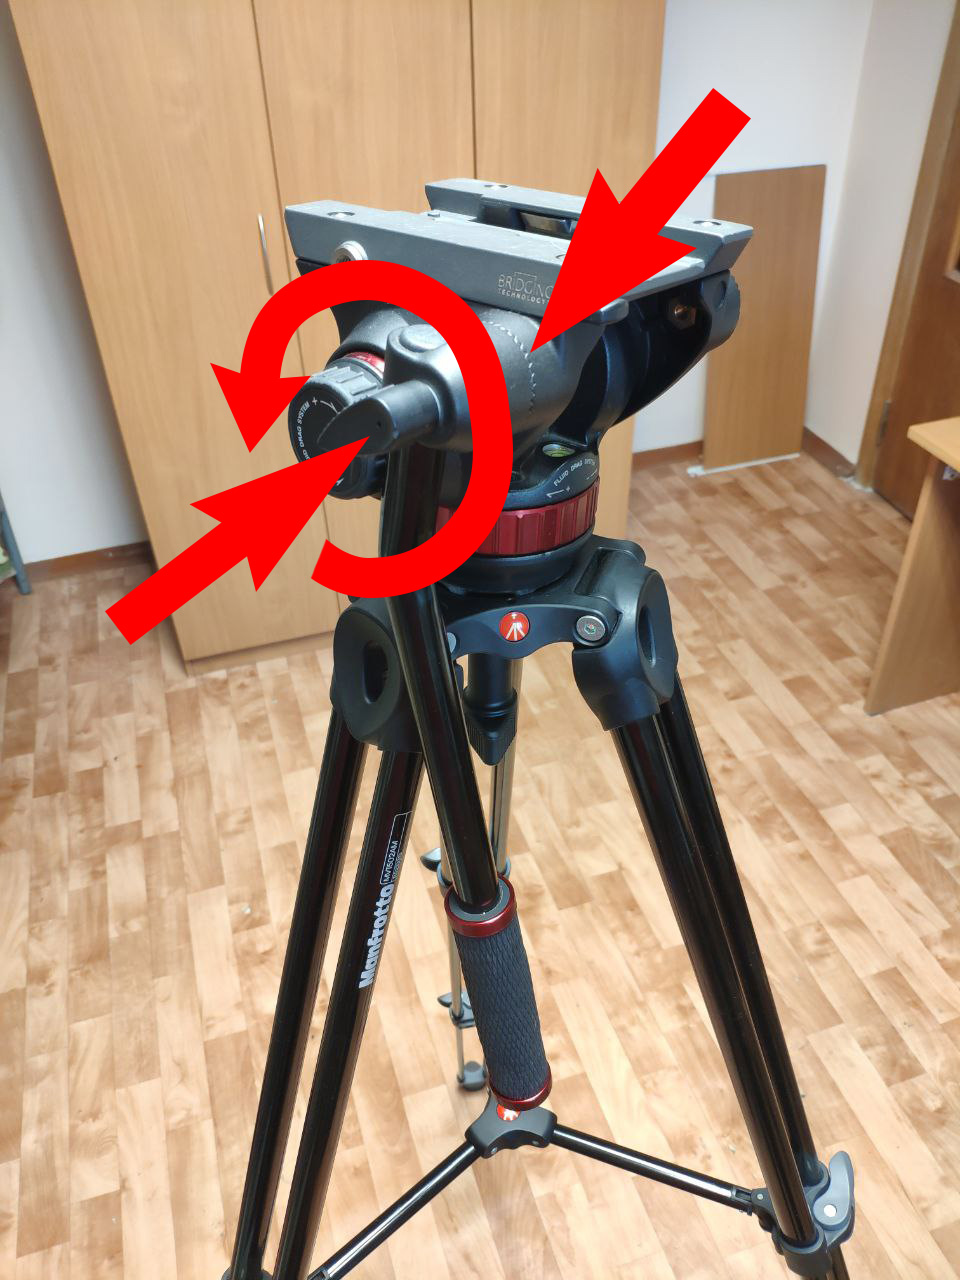
\includegraphics[width=\textwidth]{PortableCamera/tripod/step2.3-1-handle-folded.jpg}
                \end{minipage}
                \hfill
                \begin{minipage}[c]{0.43\textwidth}
                  \centering
                  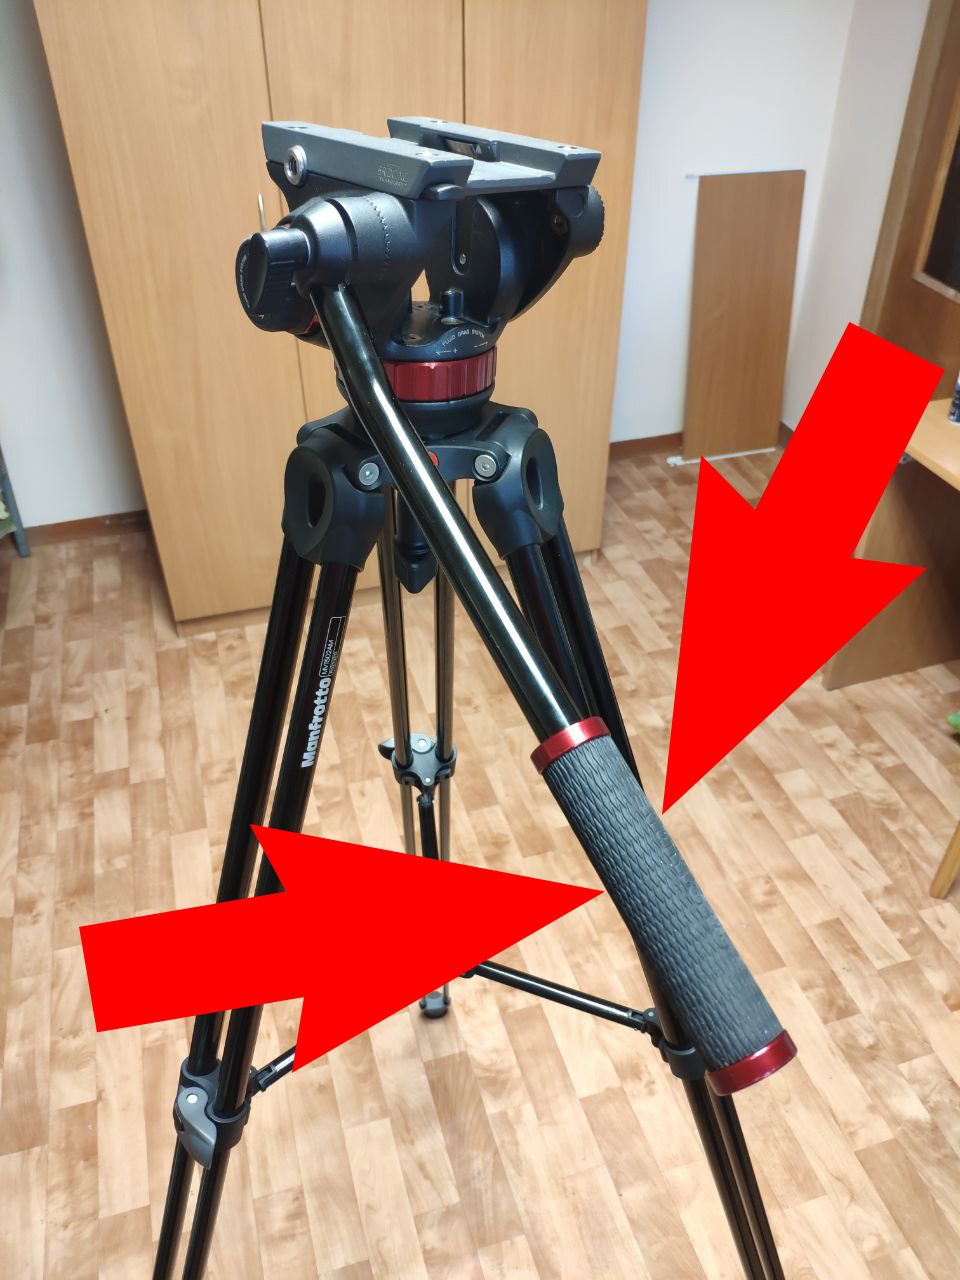
\includegraphics[width=\textwidth]{PortableCamera/tripod/step2.3-2-handle-ready.jpg}
                \end{minipage}

          \item Выровнять штатив по зелёному пузырьковому уровню.
                \par Нужно, чтобы пузырёк попал в середину. Для регулировки нужно открутить зажим под головой штатива (смотри рисунок).

                \begin{minipage}[c]{0.29\textwidth}
                  \centering
                  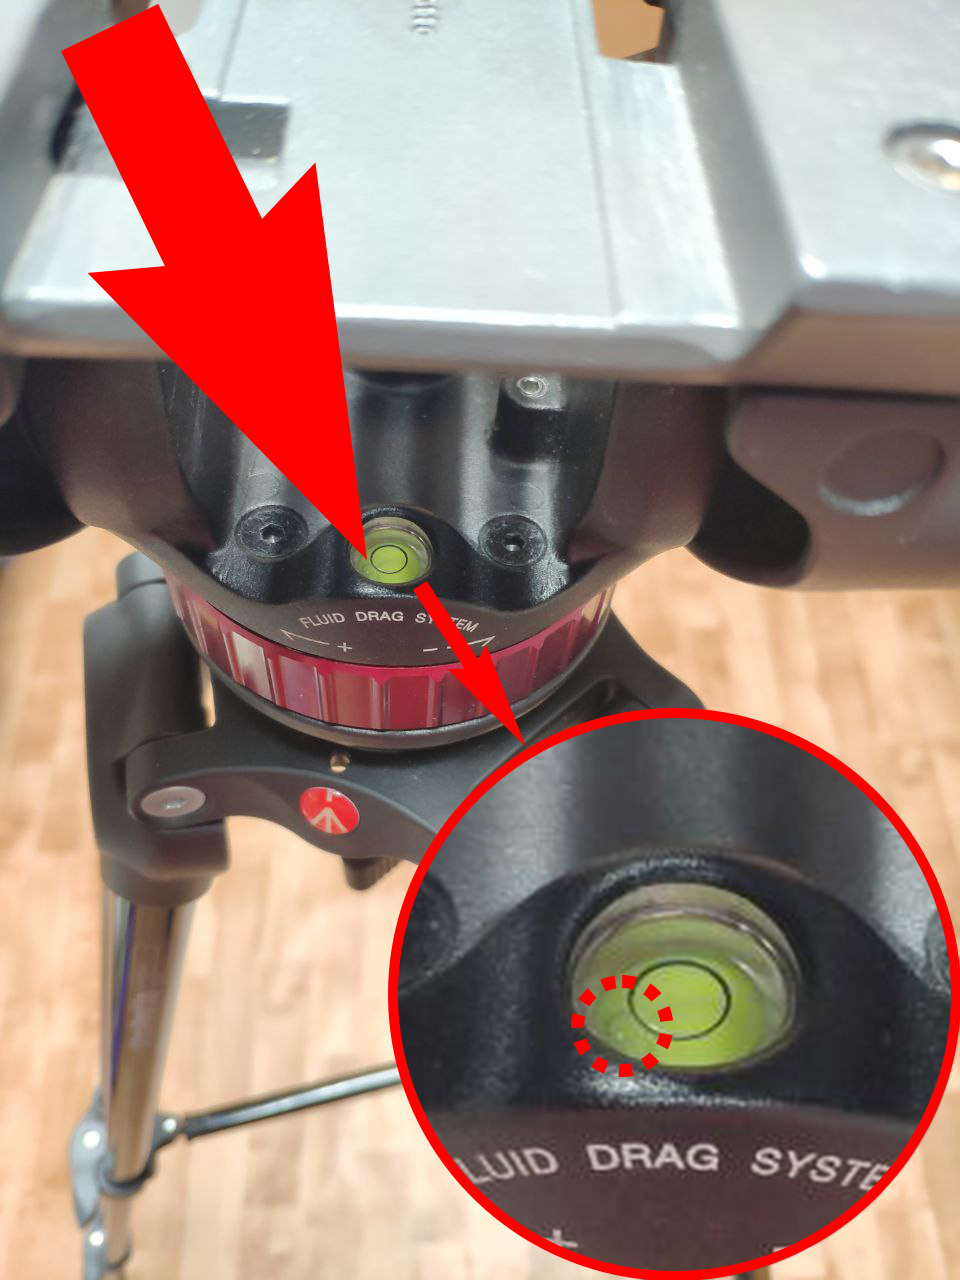
\includegraphics[width=\textwidth]{Images/PortableCamera/tripod/step2.4-1-bubble-before.jpg}
                \end{minipage}
                \hfill
                \begin{minipage}[c]{0.29\textwidth}
                  \centering
                  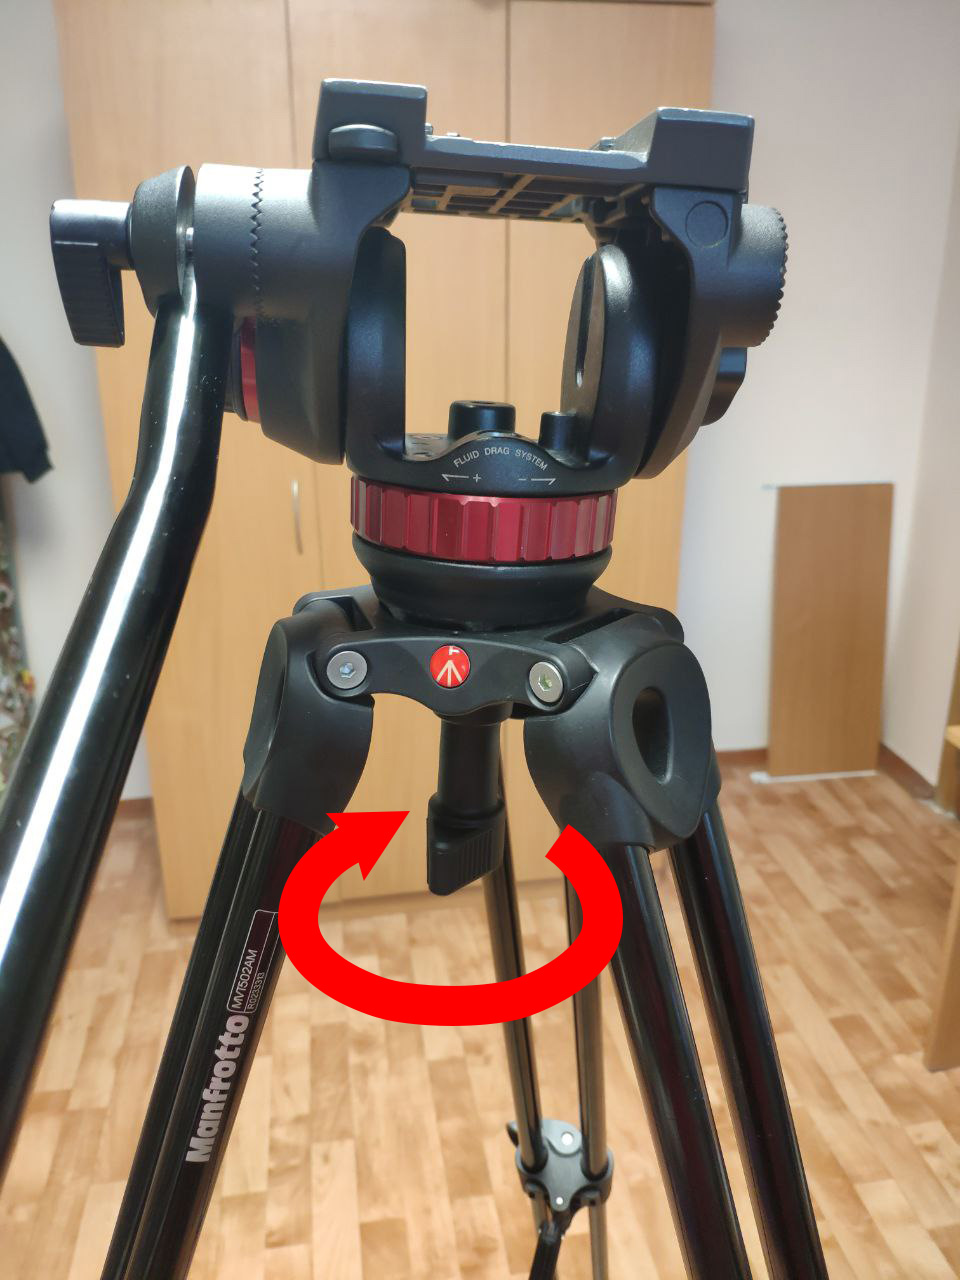
\includegraphics[width=\textwidth]{Images/PortableCamera/tripod/step2.4-2-bowl-clamp.jpg}
                \end{minipage}
                \hfill
                \begin{minipage}[c]{0.29\textwidth}
                  \centering
                  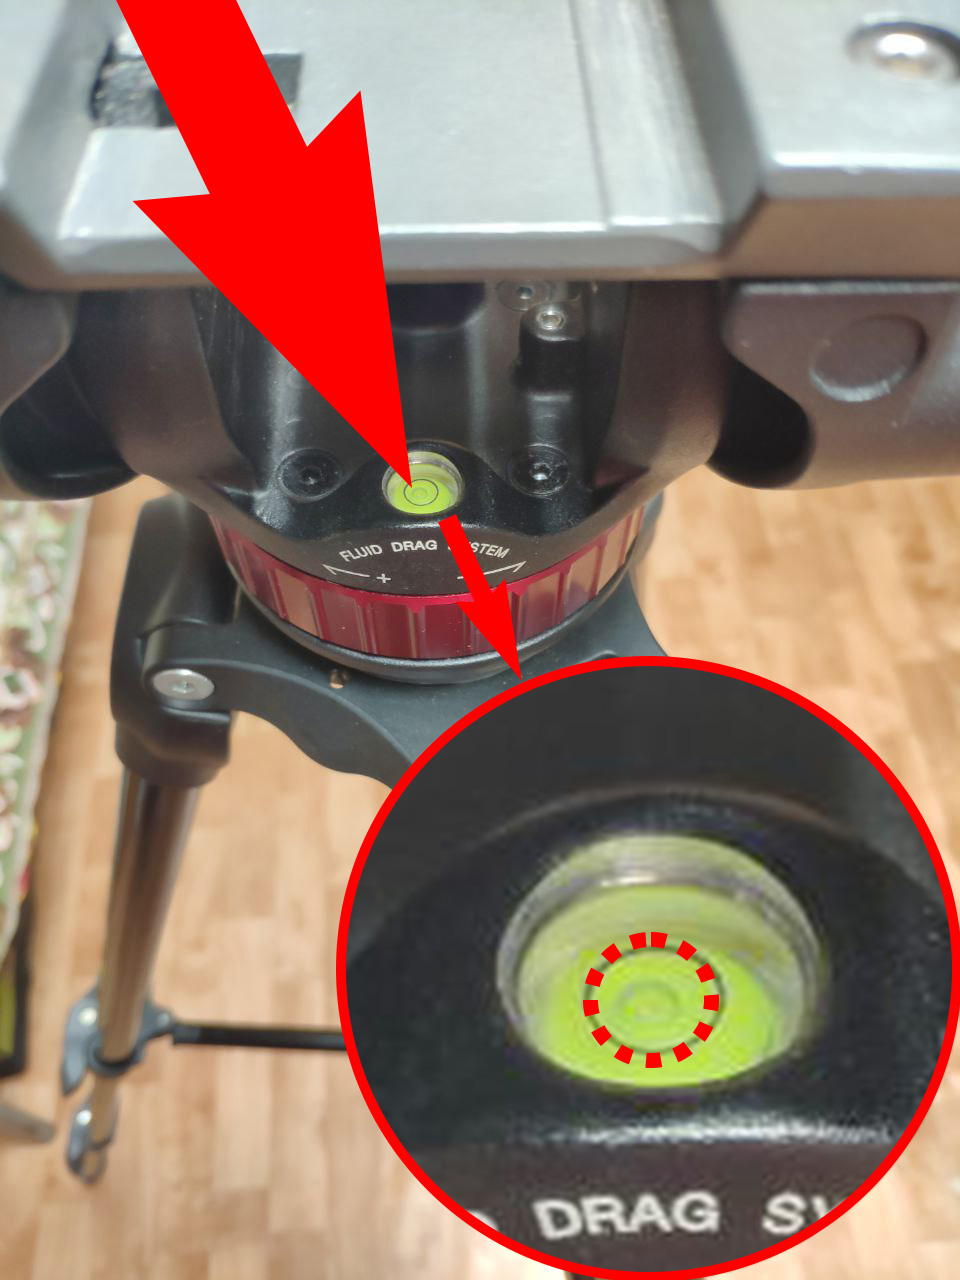
\includegraphics[width=\textwidth]{Images/PortableCamera/tripod/step2.4-3-bubble-ready.jpg}
                \end{minipage}

          \item Выровнять штатив в вертикальной плоскости.
                \par Для этого нужно воспользоваться зажимом с надписью \mitem{lock} (смотри картинку). Откручивается он против часовой стрелки. Колесо с другой стороны, подписанная \mitem{FLUID DRAG SYSTEM}, регулирует степень жесткости поворота штатива \textbf{в вертикальной плоскости}. Колесо стоит ослабить только в том случае, если после поворота зажима движение в вертикальной плоскости идёт туго. После регулировки нужно обратно закрутить зажим, чтобы \textbf{во время съёмки} лекции камера могла двигаться \textbf{только в стороны}\footnote{Если есть необходимость периодически поворачивать камеру вверх-вниз (на презентацию и на доску/лектора, например), то лучше воспользоваться связкой OBS $+$ камера --- камера снимает только доску, презентация передаётся через пирамидку. Подробнее смотри соответствующий раздел.\nopartodo{Сделать ссылку на раздел}.}.

                \begin{minipage}[c]{0.29\textwidth}
                  \centering
                  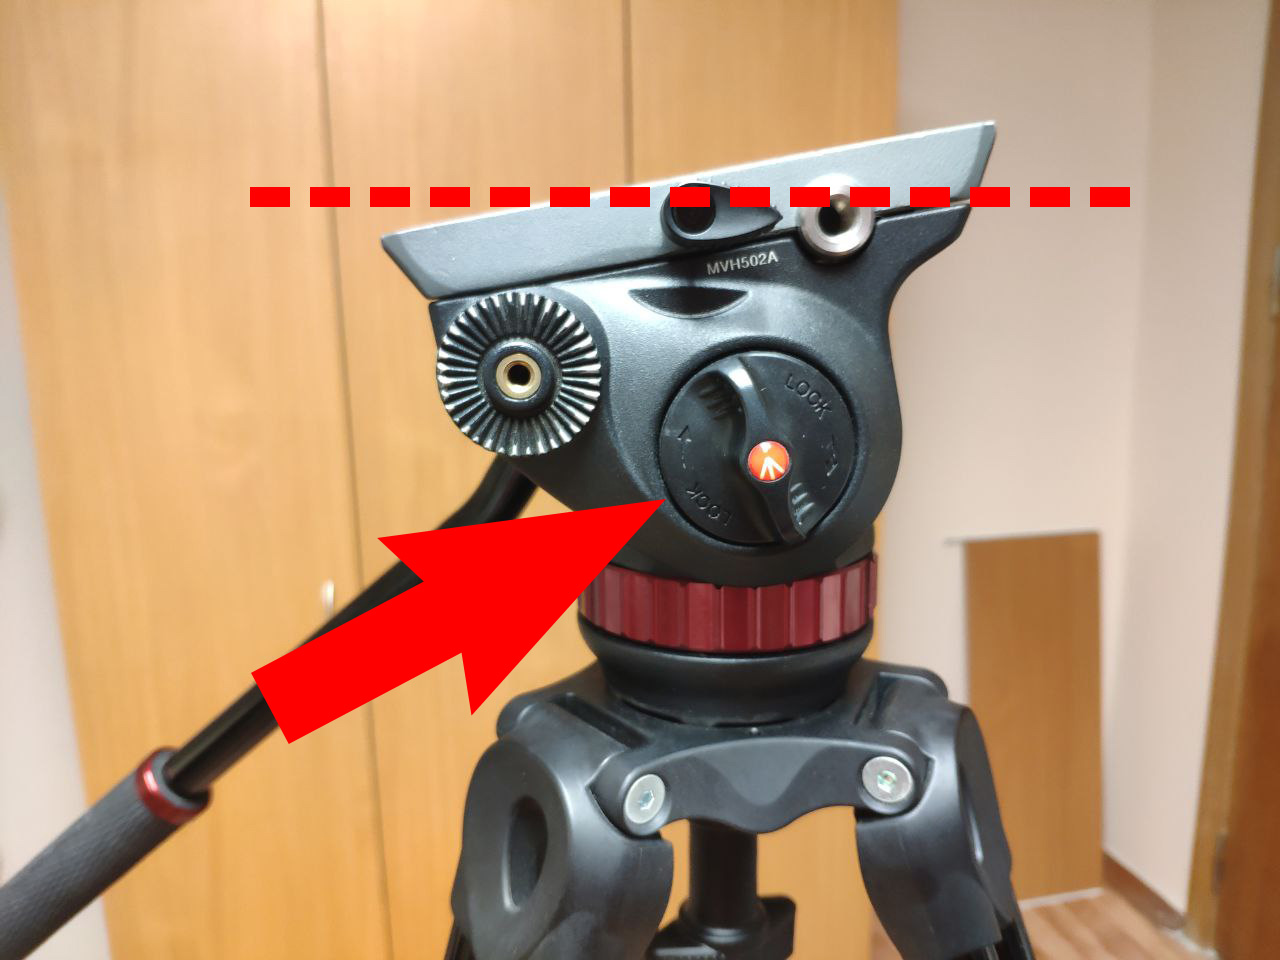
\includegraphics[width=\textwidth]{Images/PortableCamera/tripod/step2.5-1-lock.jpg}
                \end{minipage}
                \hfill
                \begin{minipage}[c]{0.29\textwidth}
                  \centering
                  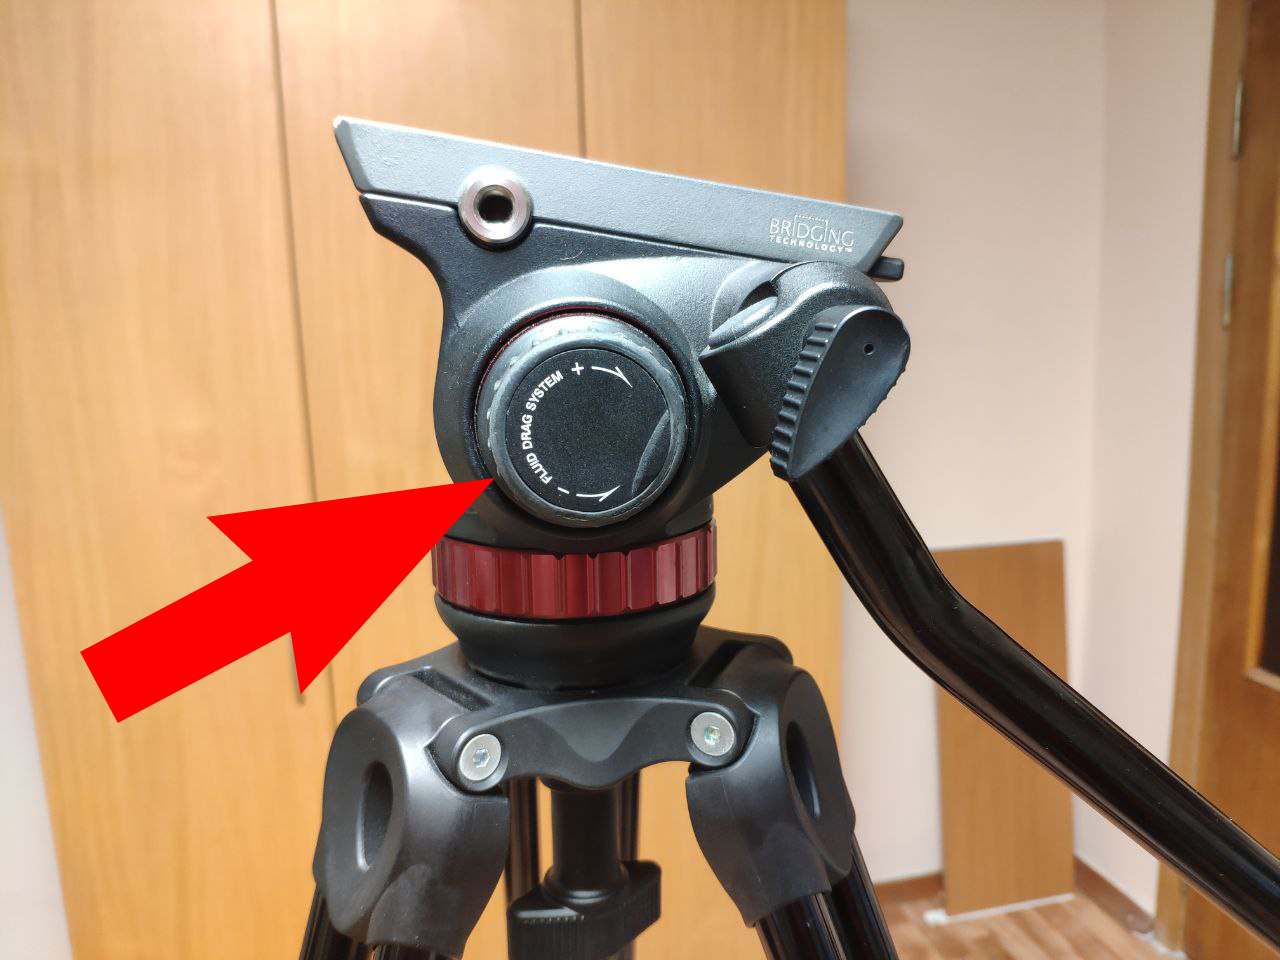
\includegraphics[width=\textwidth]{Images/PortableCamera/tripod/step2.5-2-vertical-circle.jpg}
                \end{minipage}
                \hfill
                \begin{minipage}[c]{0.29\textwidth}
                  \centering
                  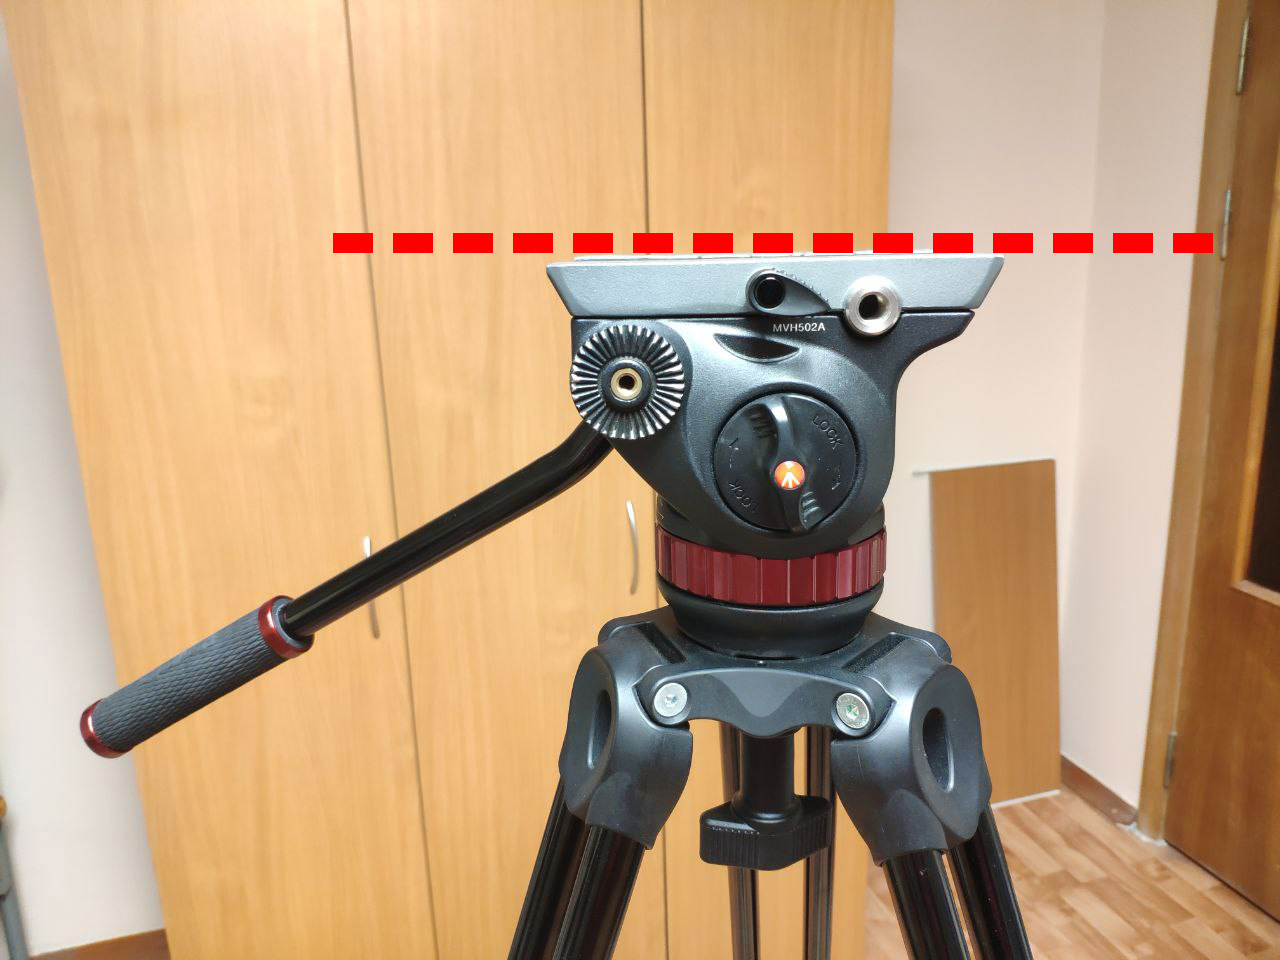
\includegraphics[width=\textwidth]{Images/PortableCamera/tripod/step2.5-3-vertical-aligned.jpg}
                \end{minipage}
        \end{enumerate}

  \item Достать камеру из портфеля.
        \par \textbf{ПОЛОЖИТЬ ПОРТФЕЛЬ НА СПИНКУ} (чтобы после открытия он лежал, как на \hyperref[fig:bag-open]{фото со стрелками}) и только из этого положения расстёгивать отдел. Если открыть портфель из стоячего положения, из него могут вывалиться петлички.

  \item Поставить камеру на штатив.
        \par Для этого надо немного открутить фиксатор 1 на картинке (против часовой стрелки), зажать чёрную кнопку 2 и вставить камеру в соответствующий паз. После чего нужно выровнять камеру по линии, отпустить кнопку и закрутить фиксатор (\textbf{не зажимать его слишком сильно!}).

        \begin{minipage}[c]{0.31\textwidth}\label{fig:retainer}
          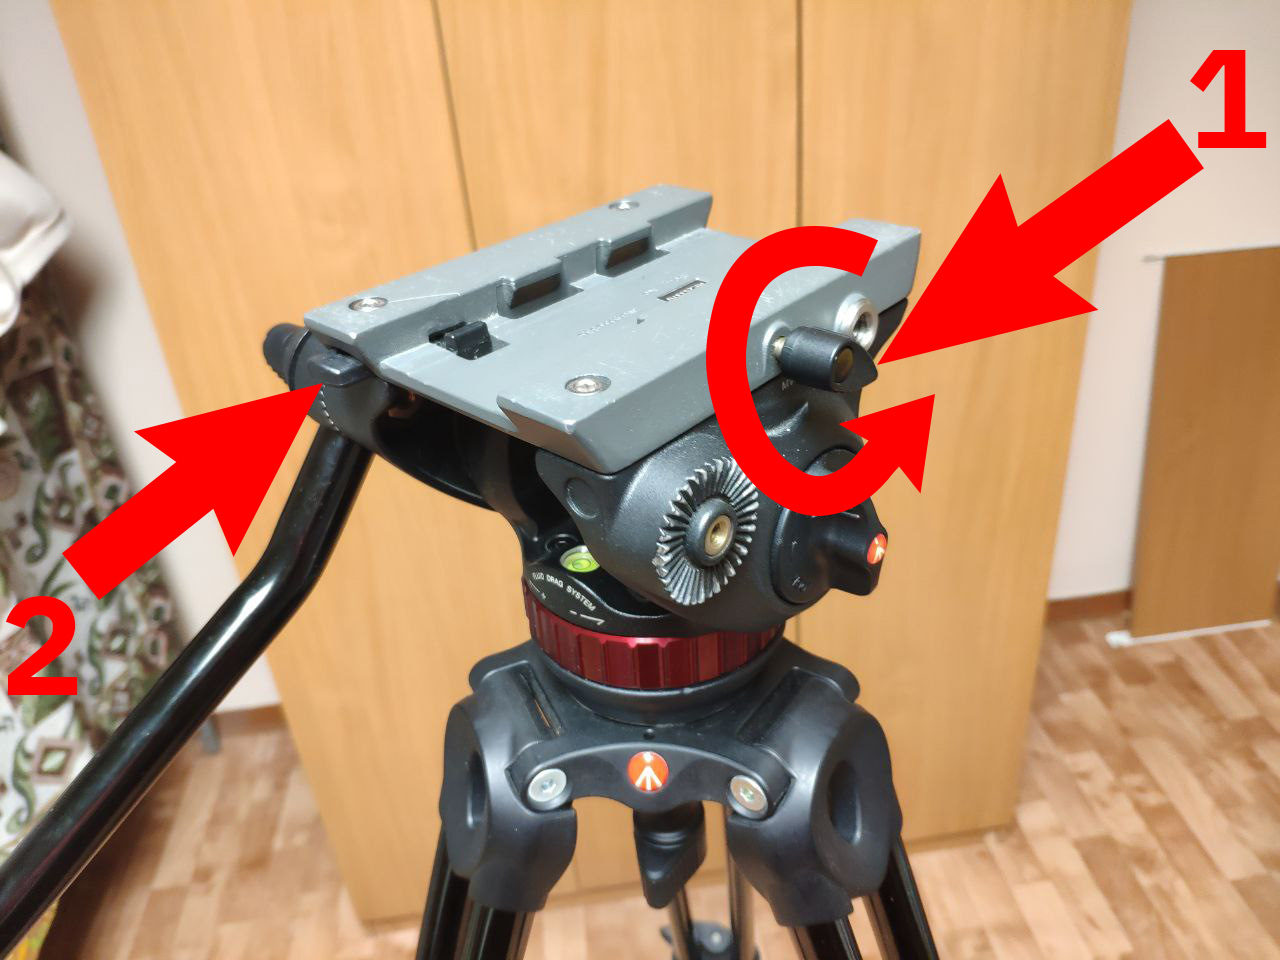
\includegraphics[width=\textwidth]{Images/PortableCamera/tripod/step3-1-retainer.jpg}
        \end{minipage}
        \hfill
        \begin{minipage}[c]{0.31\textwidth}
          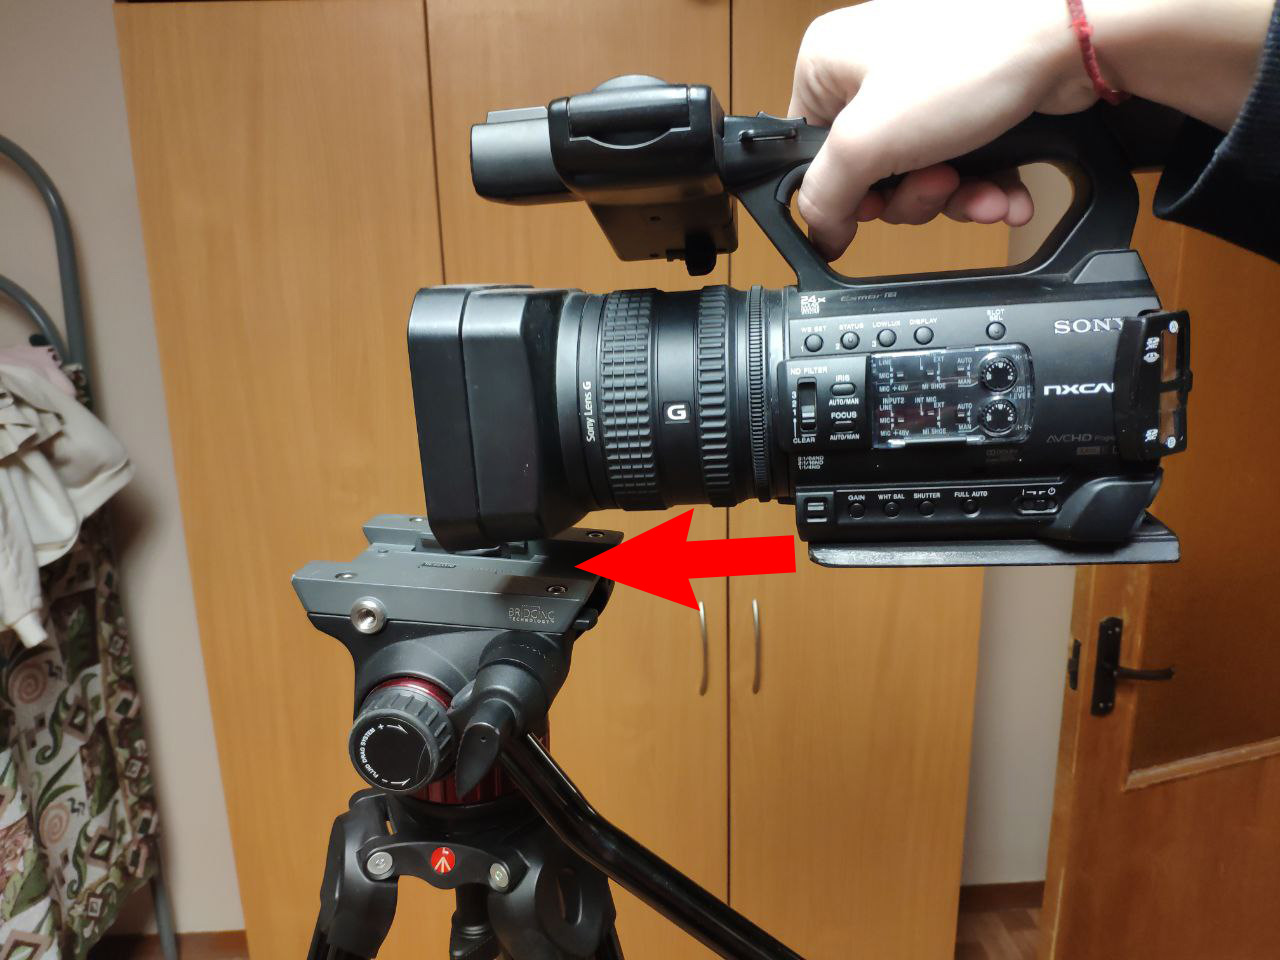
\includegraphics[width=\textwidth]{Images/PortableCamera/tripod/step3-2-camera-direction.jpg}
        \end{minipage}
        \hfill
        \begin{minipage}[c]{0.31\textwidth}
          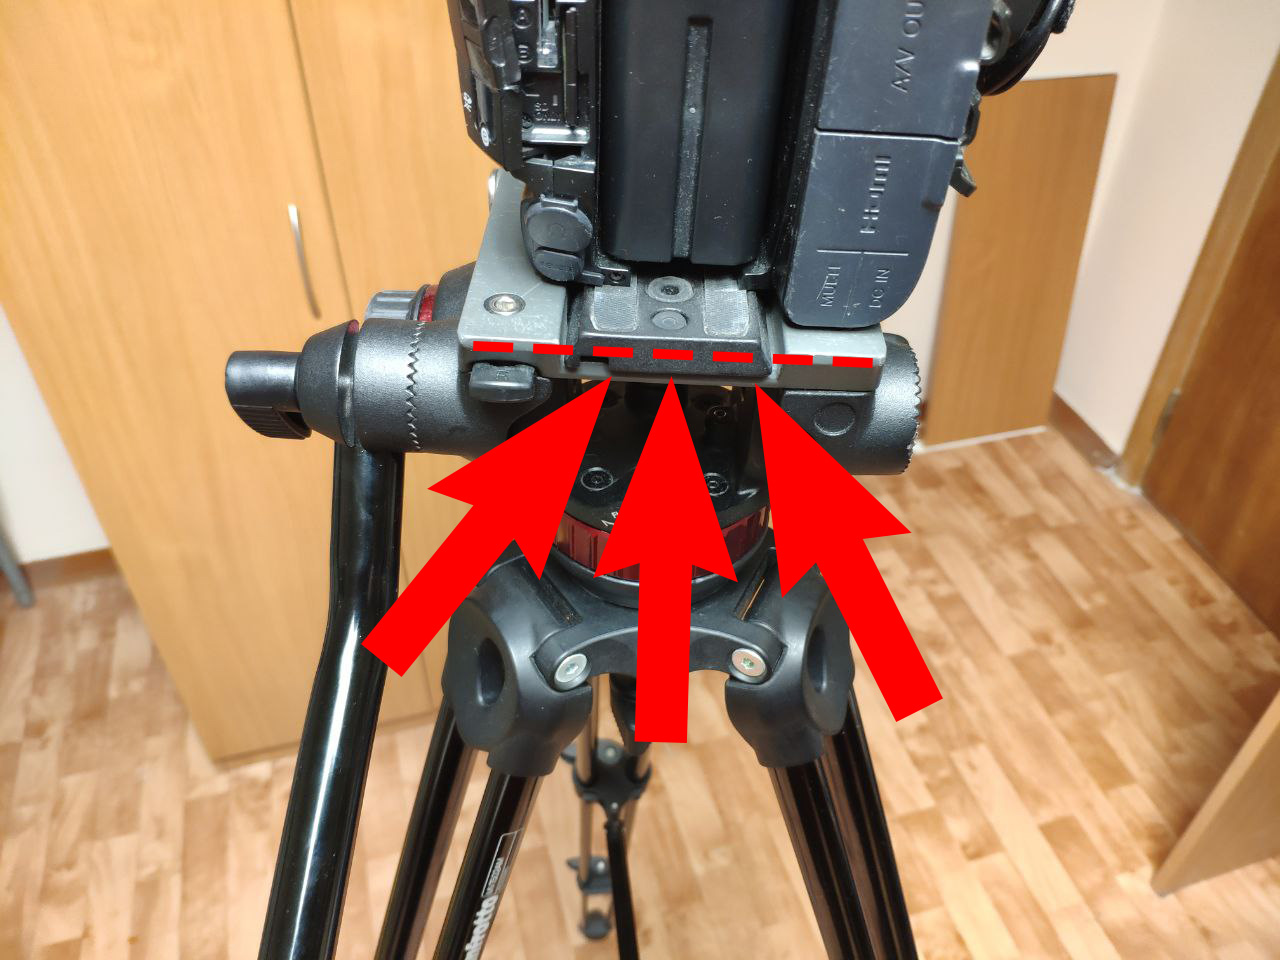
\includegraphics[width=\textwidth]{Images/PortableCamera/tripod/step3-3-camera-aligned.jpg}
        \end{minipage}

  \item Настроить (при необходимости) жёсткость поворота камеры в стороны.
        \par Красное колесо под надписью \textsf{FLUID DRAG SYSTEM} регулирует степень жёсткости поворота штатива \textbf{в стороны}. Поворот в сторону <<$-$>> делает ход более мягким.

        \begin{center}
          \begin{minipage}[c]{0.35\textwidth}
            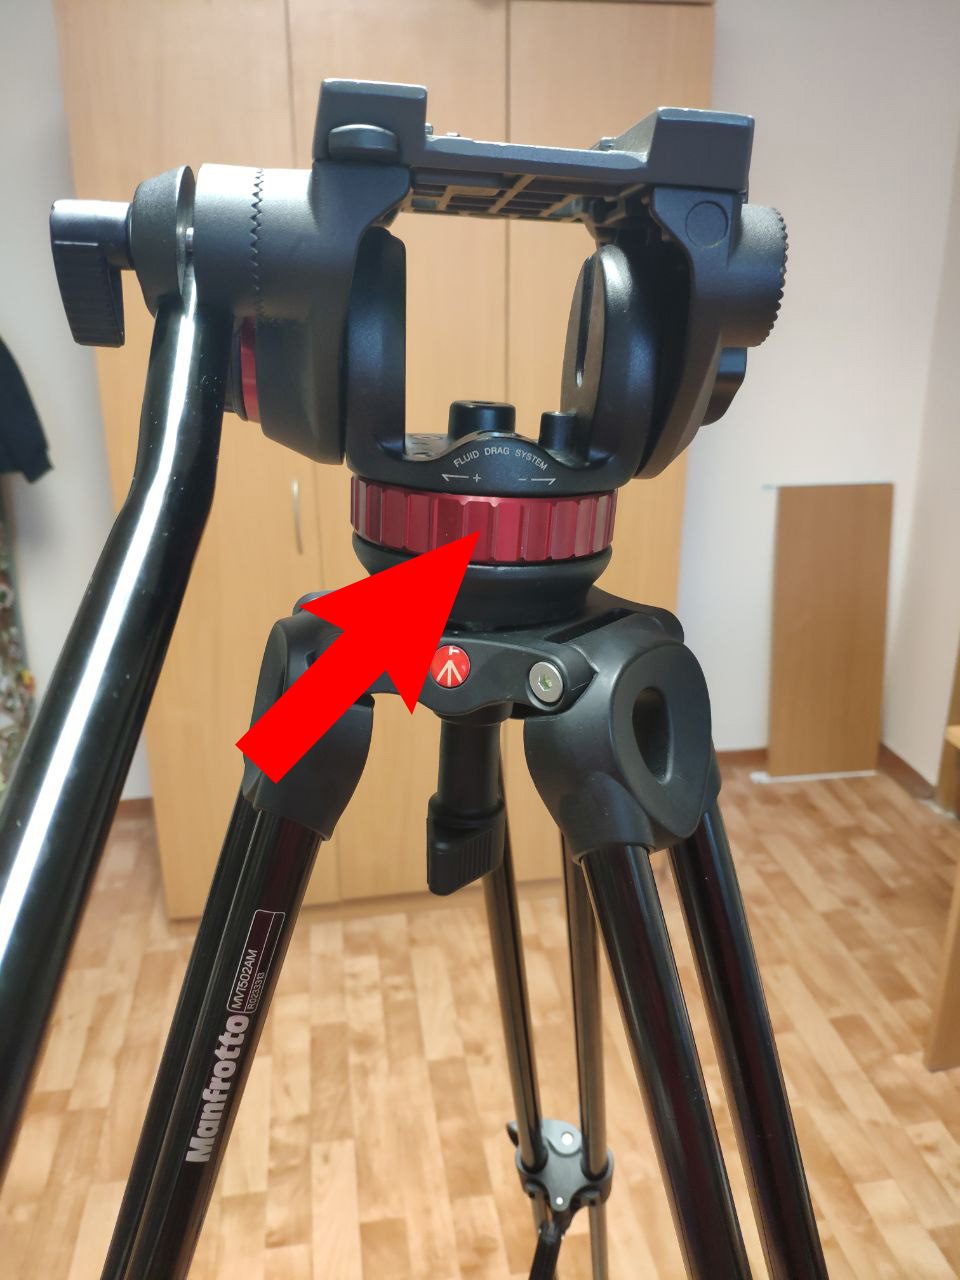
\includegraphics[width=\textwidth]{Images/PortableCamera/tripod/step4-turn-circle.jpg}
          \end{minipage}
        \end{center}

  \item Открыть окошко камеры, отогнув его влево и повернув на себя. Включить камеру.

        \begin{minipage}[c]{0.45\textwidth}
          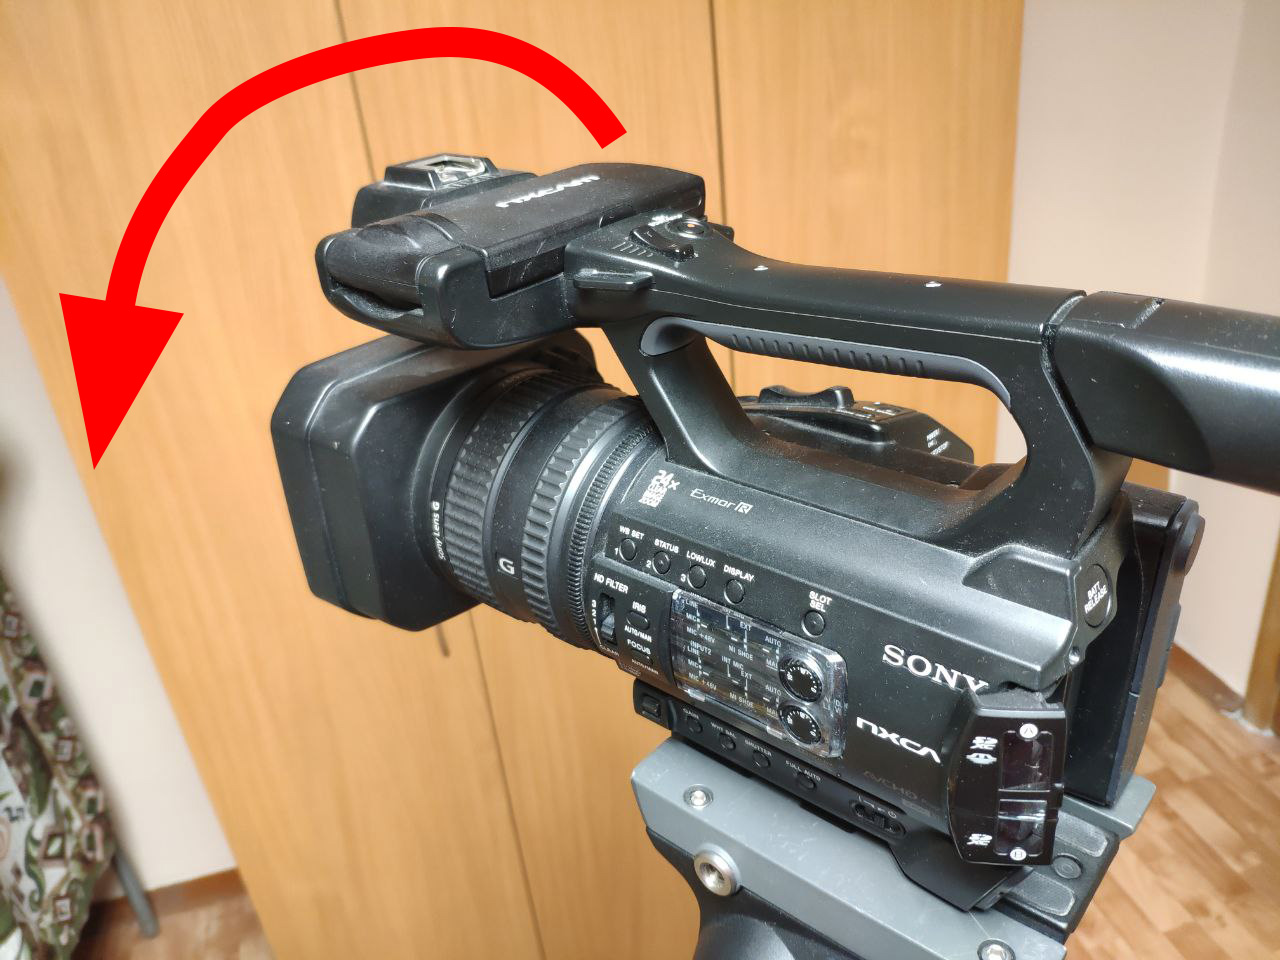
\includegraphics[width=\textwidth]{Images/PortableCamera/tripod/step5-1-window-off.jpg}
        \end{minipage}
        \hfill
        \begin{minipage}[c]{0.45\textwidth}
          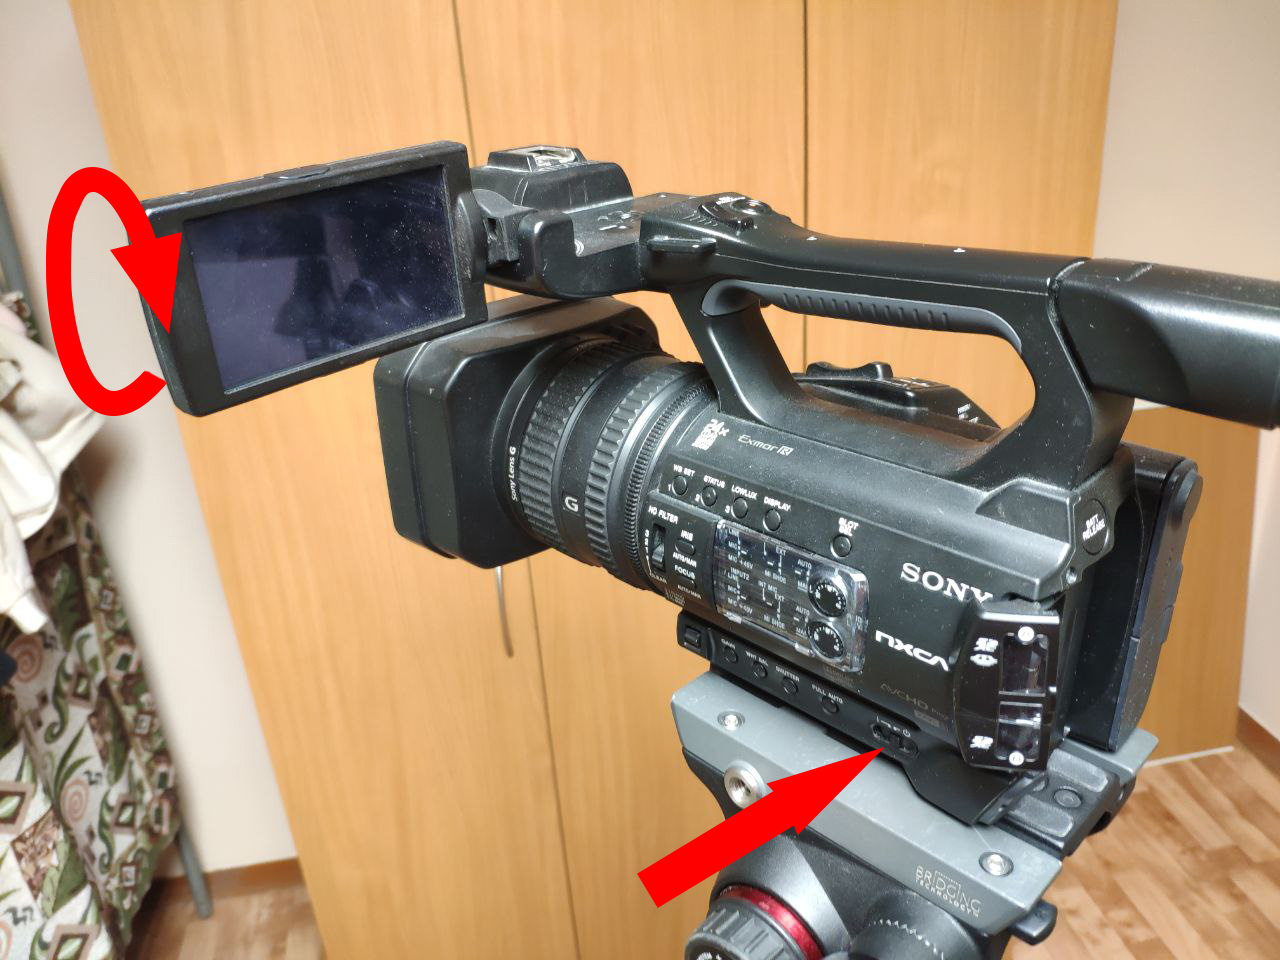
\includegraphics[width=\textwidth]{Images/PortableCamera/tripod/step5-2-window-on.jpg}
        \end{minipage}

  \item Снять крышку с объектива и \textbf{положить её в верхний карман портфеля}, чтобы не потерять.
        \par Крышка снимается путём надавливания с двух сторон, как показано на картинке. Верхний карман портфеля --- тот, где лежат петлички (\hyperref[fig:bag-open]{фото} с описанием названий карманов).

        \begin{center}
          \begin{minipage}[c]{0.4\textwidth}
            \centering
            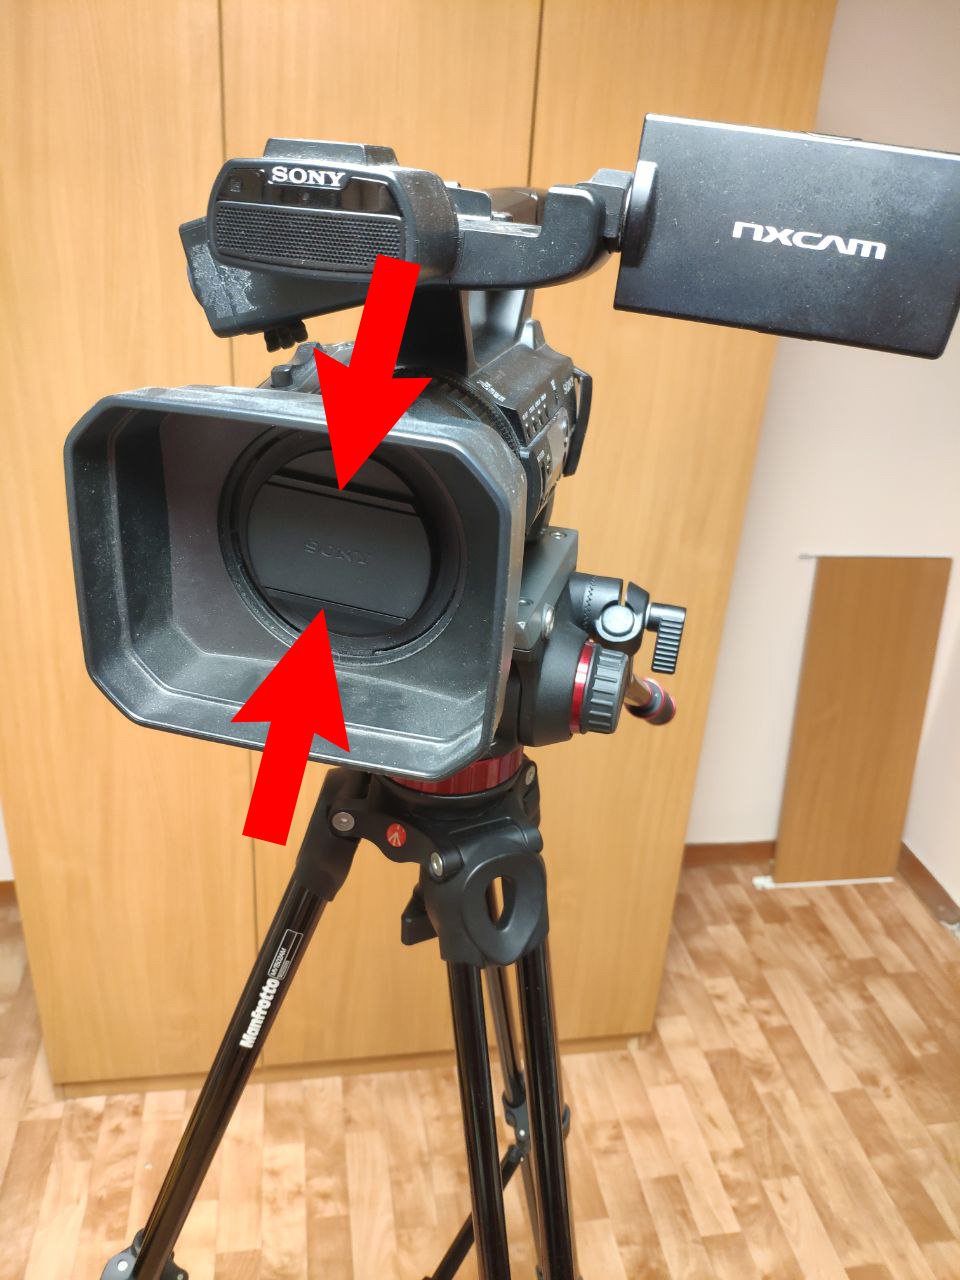
\includegraphics[width=\textwidth]{Images/PortableCamera/tripod/step6-lens-cover.jpg}
          \end{minipage}
        \end{center}

  \item Проверить, что на камере горит кнопка \mitem{full auto} и \mitem{ND Filter} стоит в положении \texttt{CLEAR}.

        \begin{center}
          \begin{minipage}[c]{0.6\textwidth}
            \centering
            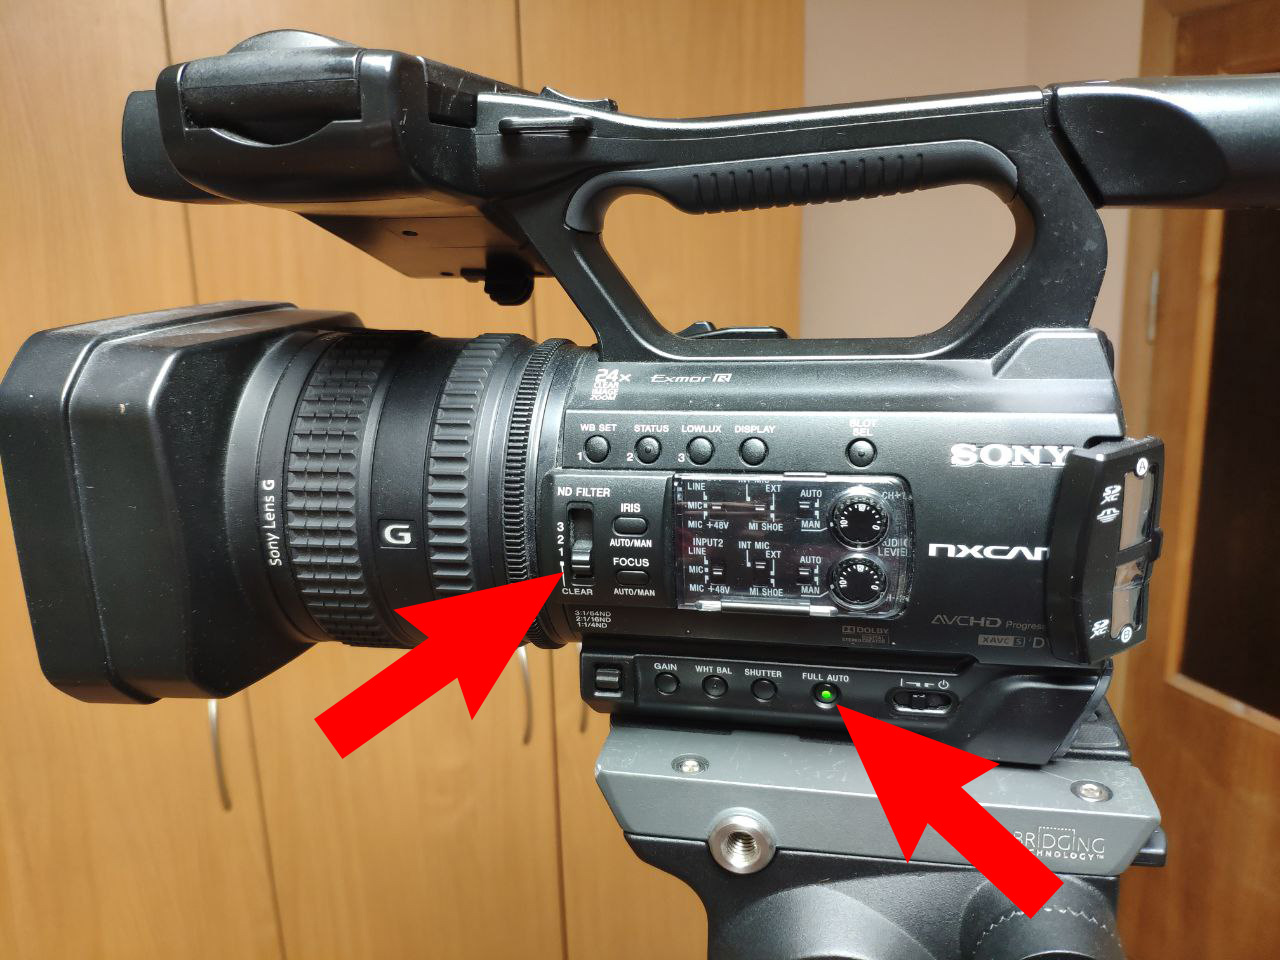
\includegraphics[width=\textwidth]{Images/PortableCamera/tripod/step7-bottons-on.jpg}
          \end{minipage}
        \end{center}

  \item Проверить заряд батареи\footnote{Если в камере большой аккум (10100 mAh), то на 1 лекцию нужно $\ge 20\%$. Если в камере стандартный аккум (3500 mAh), то на лекцию нужно $\ge 35\%$.} и количество оставшейся памяти для записи.
        \par Если чего-то не хватает, написать в чат \hyperlink{emergency-chat-vk}{emergency} и тегнуть ответственного, у которого брали камеру\footnote{Писать лучше в чат, а не в ЛС, потому что ответственный может быть занят, но помочь вам, возможно, сможет и кто-то другой.}.

        \begin{center}
          \begin{minipage}[c]{0.6\textwidth}
            \centering
            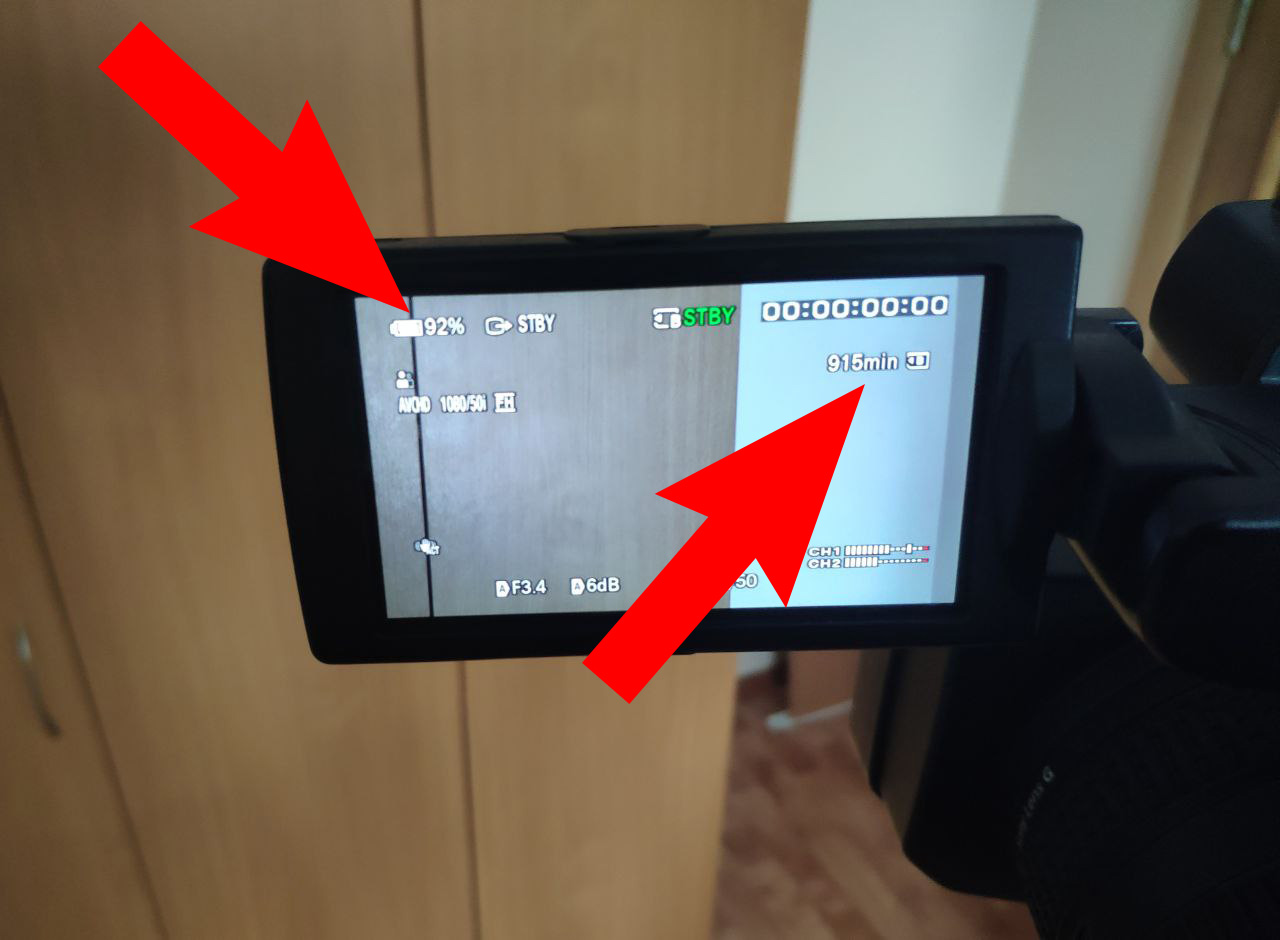
\includegraphics[width=\textwidth]{Images/PortableCamera/tripod/step8-window.jpg}
          \end{minipage}
        \end{center}

  \item (Для тех, кто пишет таймкоды) Сбросить таймлайн записи на камеру.
        \par Справа сверху в окошке есть счётчик. Он увеличивается во время записи. Для того, чтобы использовать его для написания таймкодов, нужно сбросить значение в положение 00:00:00:00. Воспользуйтей кнопками рядом с окошком просмотра: кнопка \mitem{menu} $\ra$ стрелка вниз, пока не перейдём в раздел \mitem{TC/UB SET} \ $\ra$ \ стрелка вправо \ $\ra$ \ \mitem{TC preset} \ $\ra$ кнопка \mitem{set} на камере \ $\ra$ \ \mitem{reset} \ $\ra$ \ кнопка \mitem{set} на камере \ $\ra$ \ кнопка \mitem{menu} (чтобы закрыть меню).

        \begin{minipage}[c]{0.4\textwidth}
          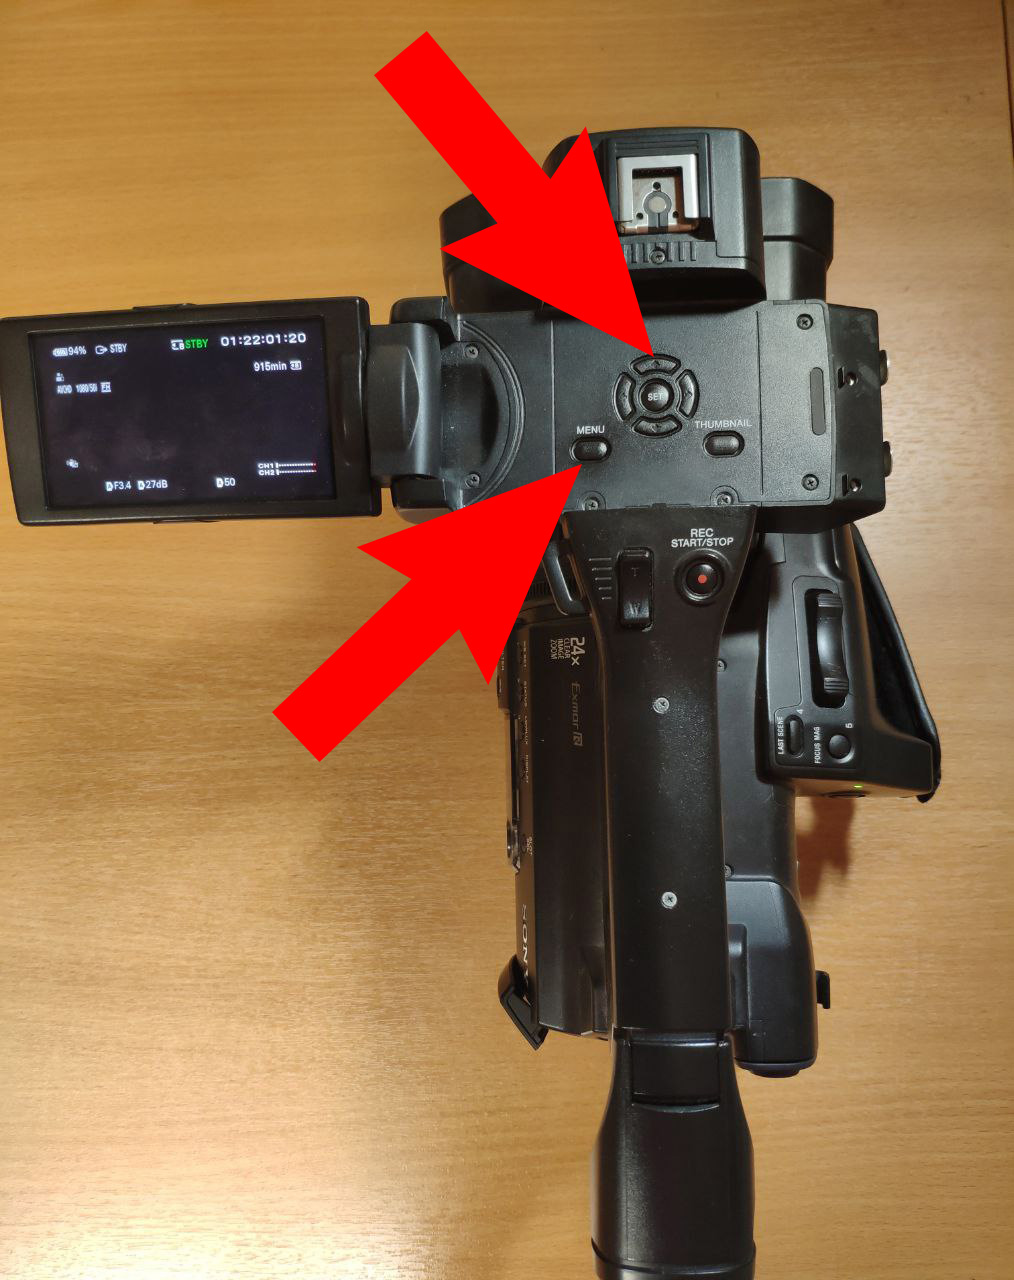
\includegraphics[width=\textwidth]{Images/PortableCamera/tripod/step9-1-view-from-above.jpg}
        \end{minipage}
        \hfill
        \begin{minipage}[c]{0.51\textwidth}
          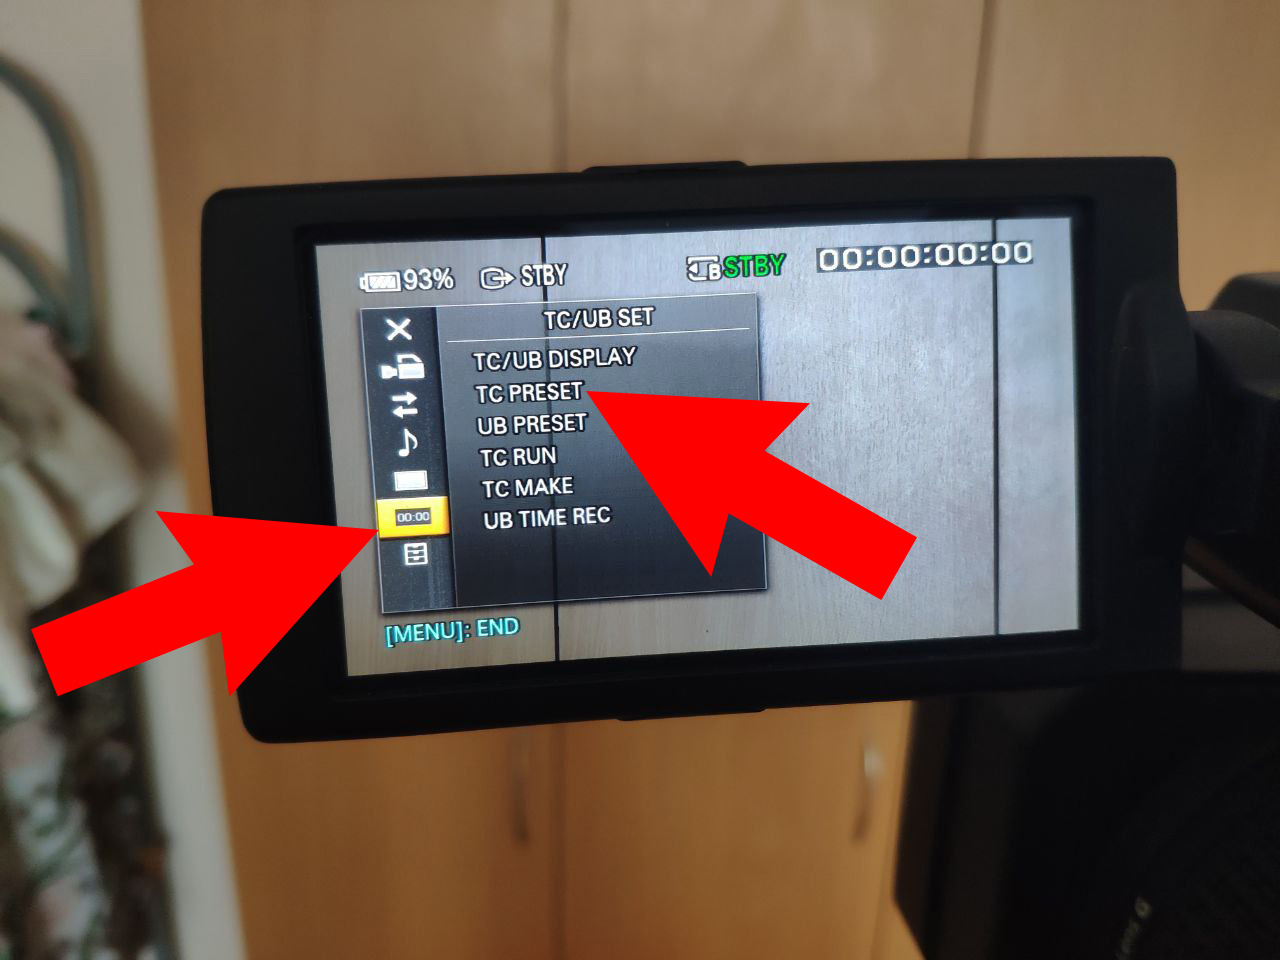
\includegraphics[width=\textwidth]{Images/PortableCamera/tripod/step9-2-camera-menu.jpg}
        \end{minipage}

  \item Подключить петличку.
        \begin{enumerate}
          \item Достать петлички из рюкзака --- они лежат в кармане с камерой справа.

          \item Определить, какую петличку отдать лектору, а какую --- подключать к камере.
                \par На задней стороне петличек можно найти названия \mitem{receiver} и \mitem{transmitter}. \mitem{receiver} подключается к камере, \mitem{transmitter} --- отдаётся лектору.

                \begin{minipage}[c]{0.4\textwidth}
                  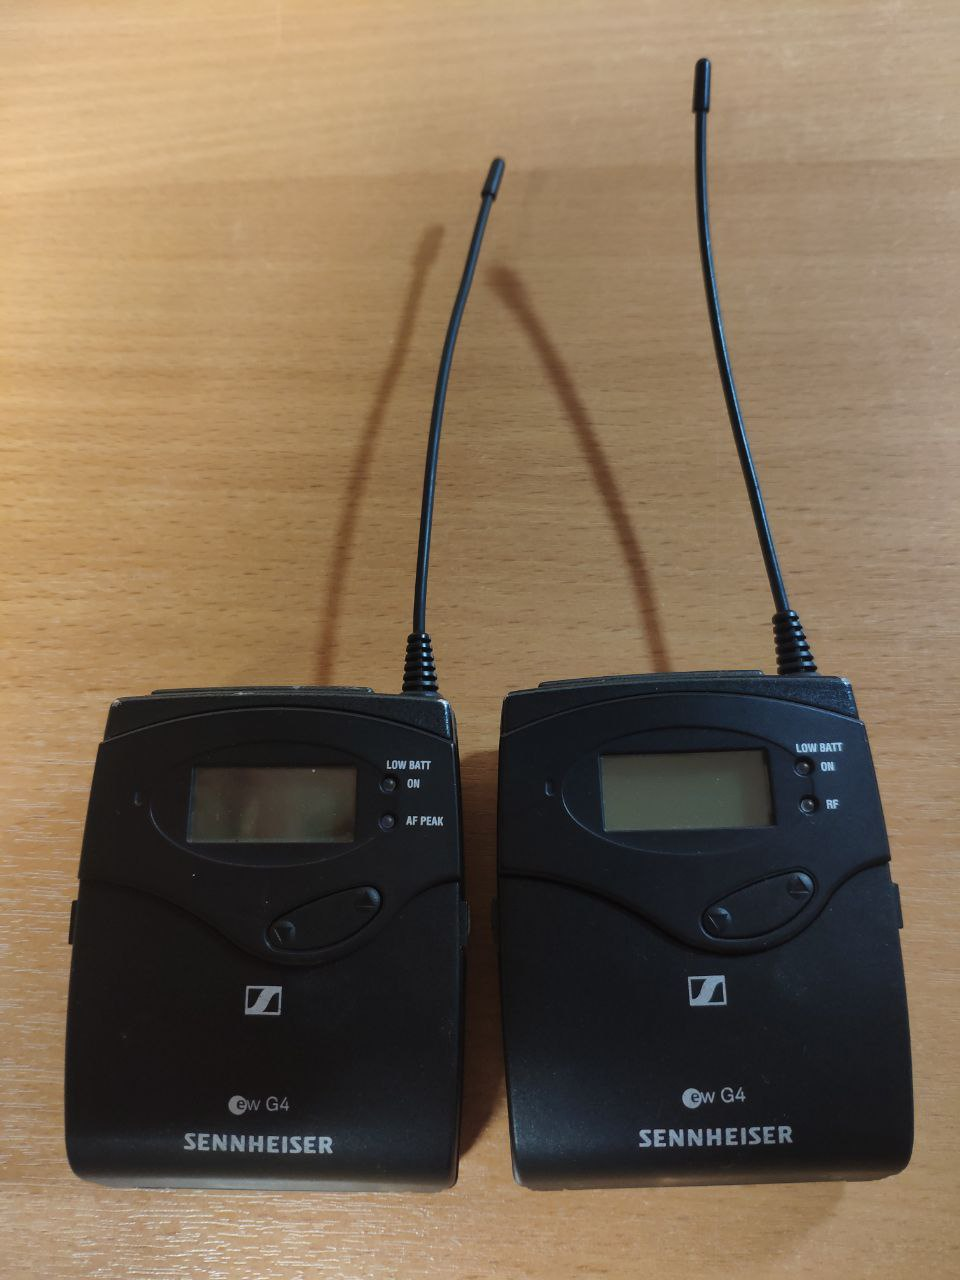
\includegraphics[width=\textwidth]{Images/PortableCamera/micro/step10.1-1-micro-diference-front.jpg}
                \end{minipage}
                \hfill
                \begin{minipage}[c]{0.4\textwidth}
                  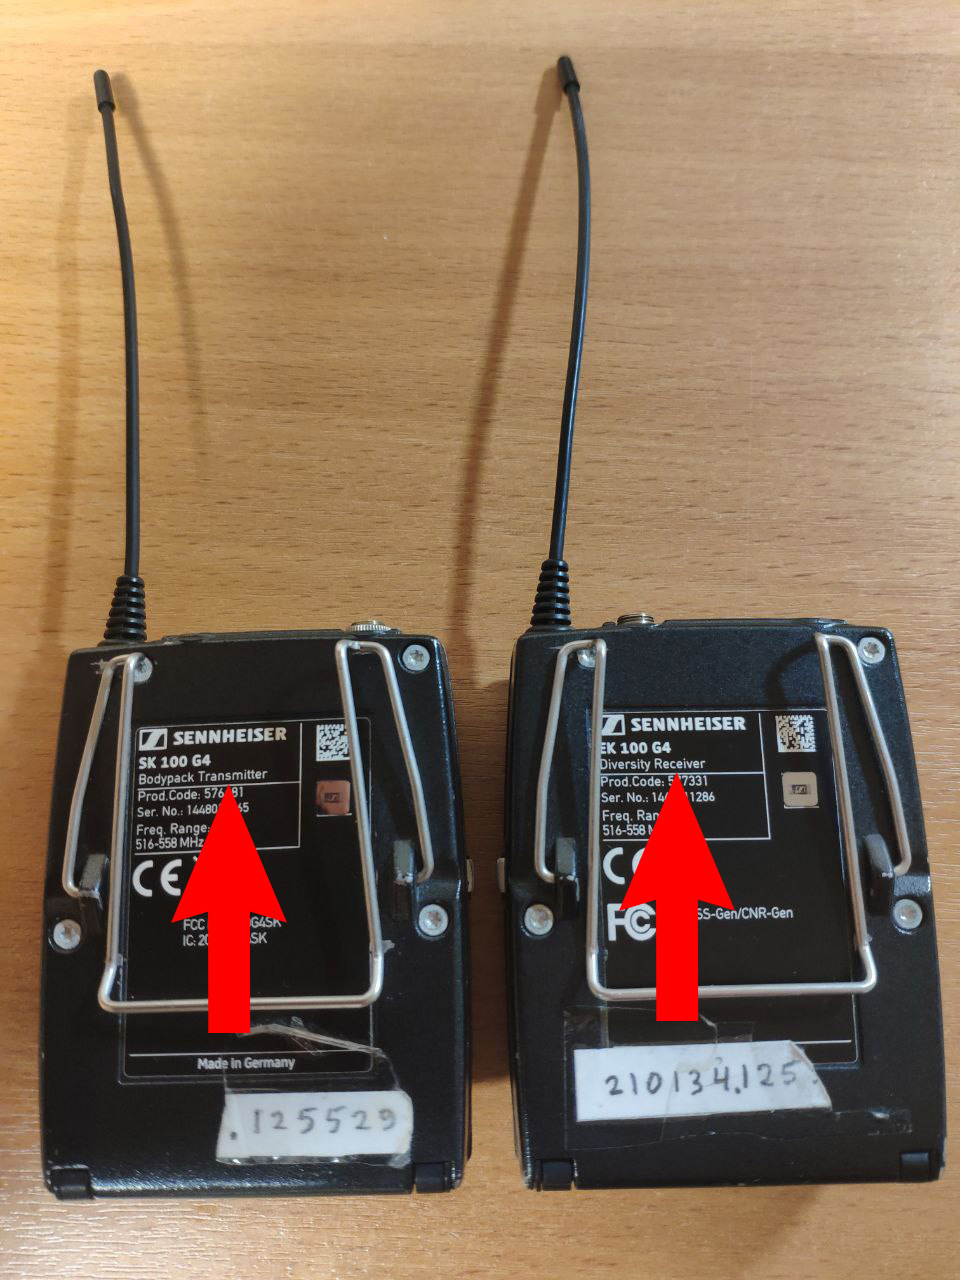
\includegraphics[width=\textwidth]{Images/PortableCamera/micro/step10.1-1-micro-diference-back.jpg}
                \end{minipage}

          \item Включить \mitem{receiver}.
                \par Для этого зажать боковые кнопки, открыть отдел с аккумами, задержать кнопку \mitem{ON/OFF} 2-3 секунды, закрыть отдел до щелчка. Если \mitem{receiver} не влючается, вставить в него запасные батарейки (лежат в нижнем кармане рюкзака --- \hyperref[fig:bag-open]{картинка}) и попробовать включить с ними.

                \begin{minipage}[c]{0.29\textwidth}
                  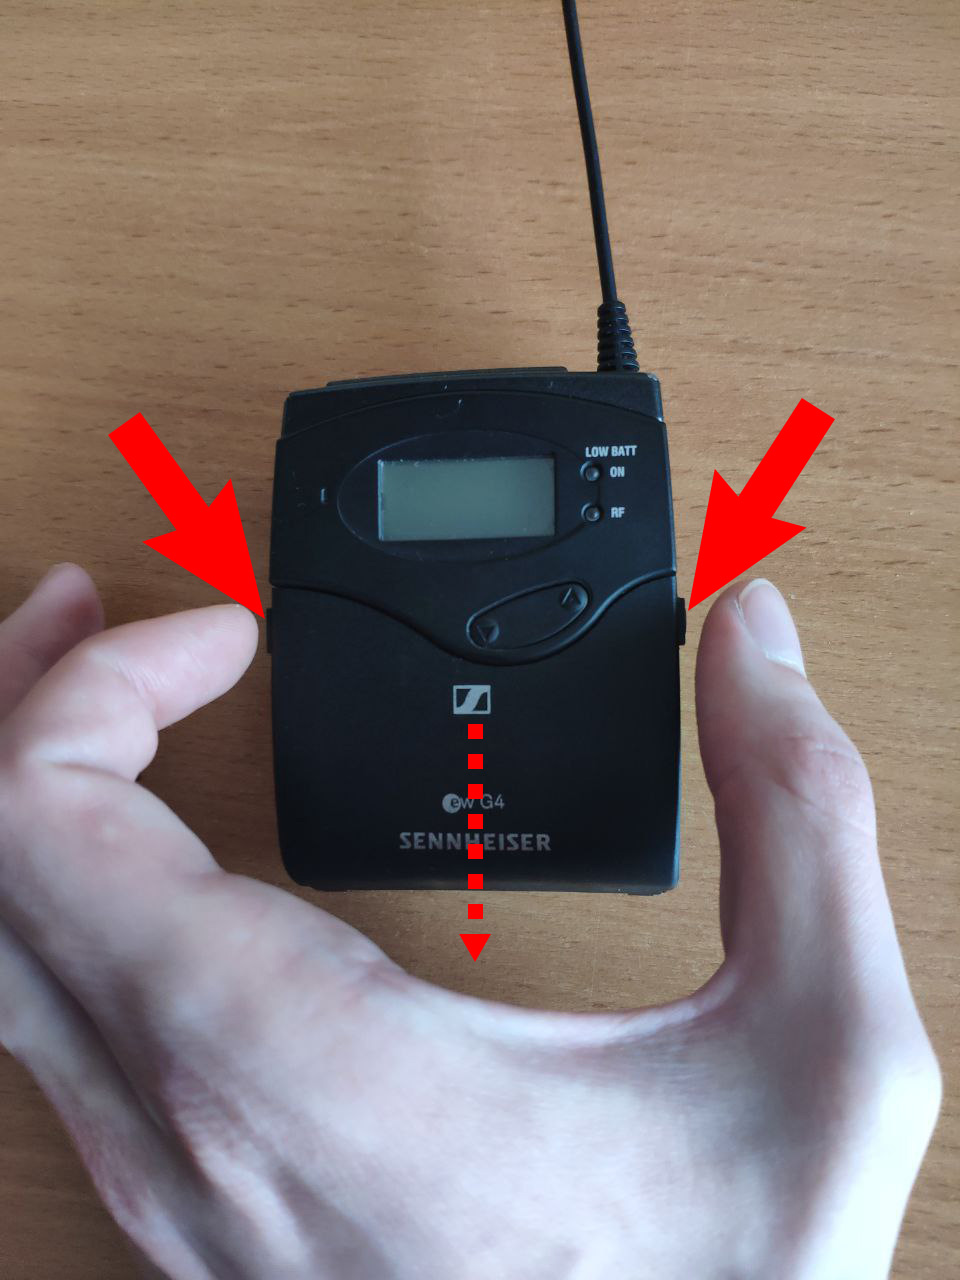
\includegraphics[width=\textwidth]{Images/PortableCamera/micro/step10.2-1-micro-open.jpg}
                \end{minipage}
                \hfill
                \begin{minipage}[c]{0.29\textwidth}
                  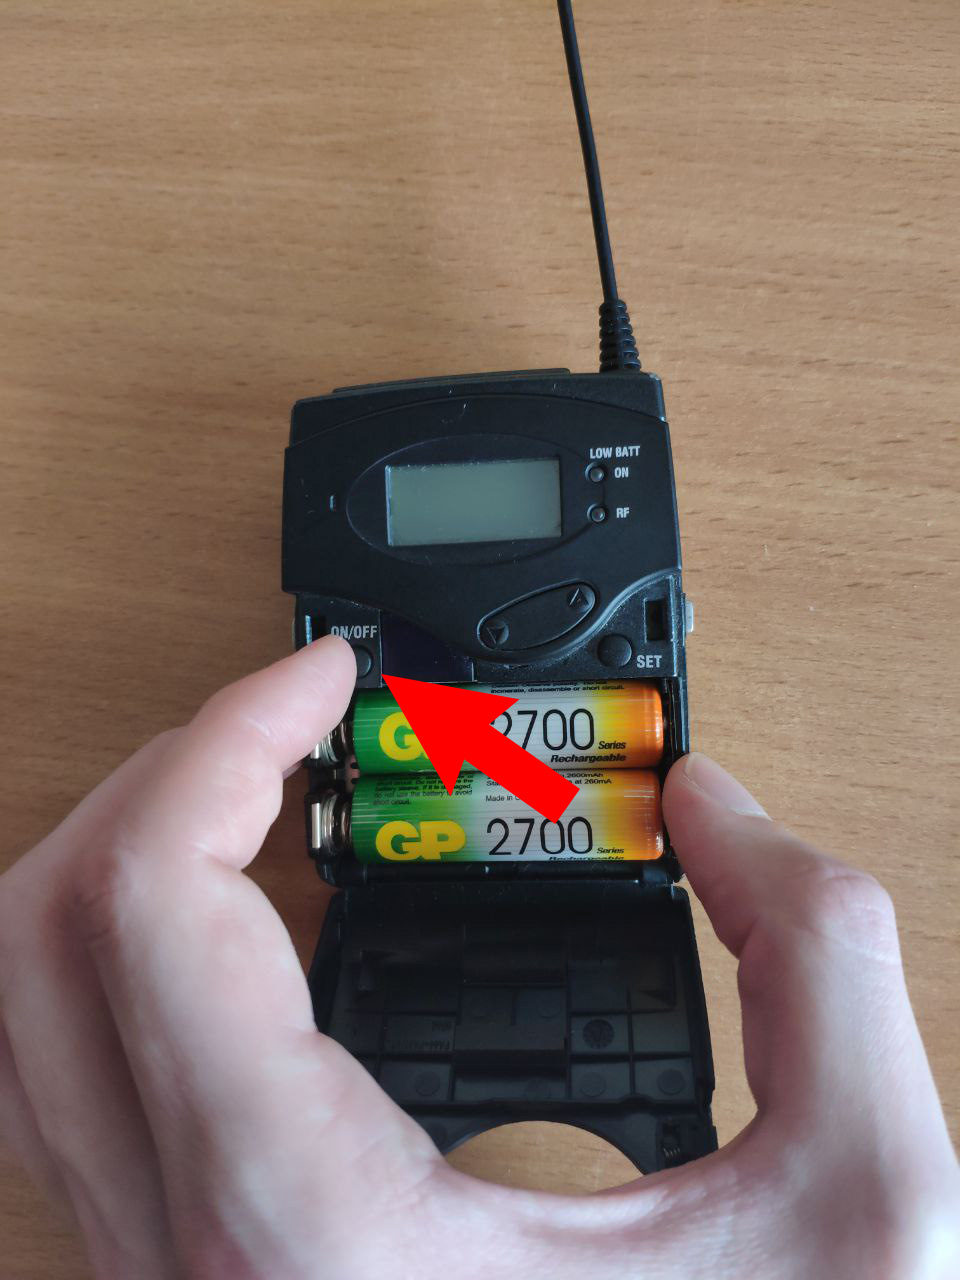
\includegraphics[width=\textwidth]{Images/PortableCamera/micro/step10.2-2-micro-off.jpg}
                \end{minipage}
                \hfill
                \begin{minipage}[c]{0.29\textwidth}
                  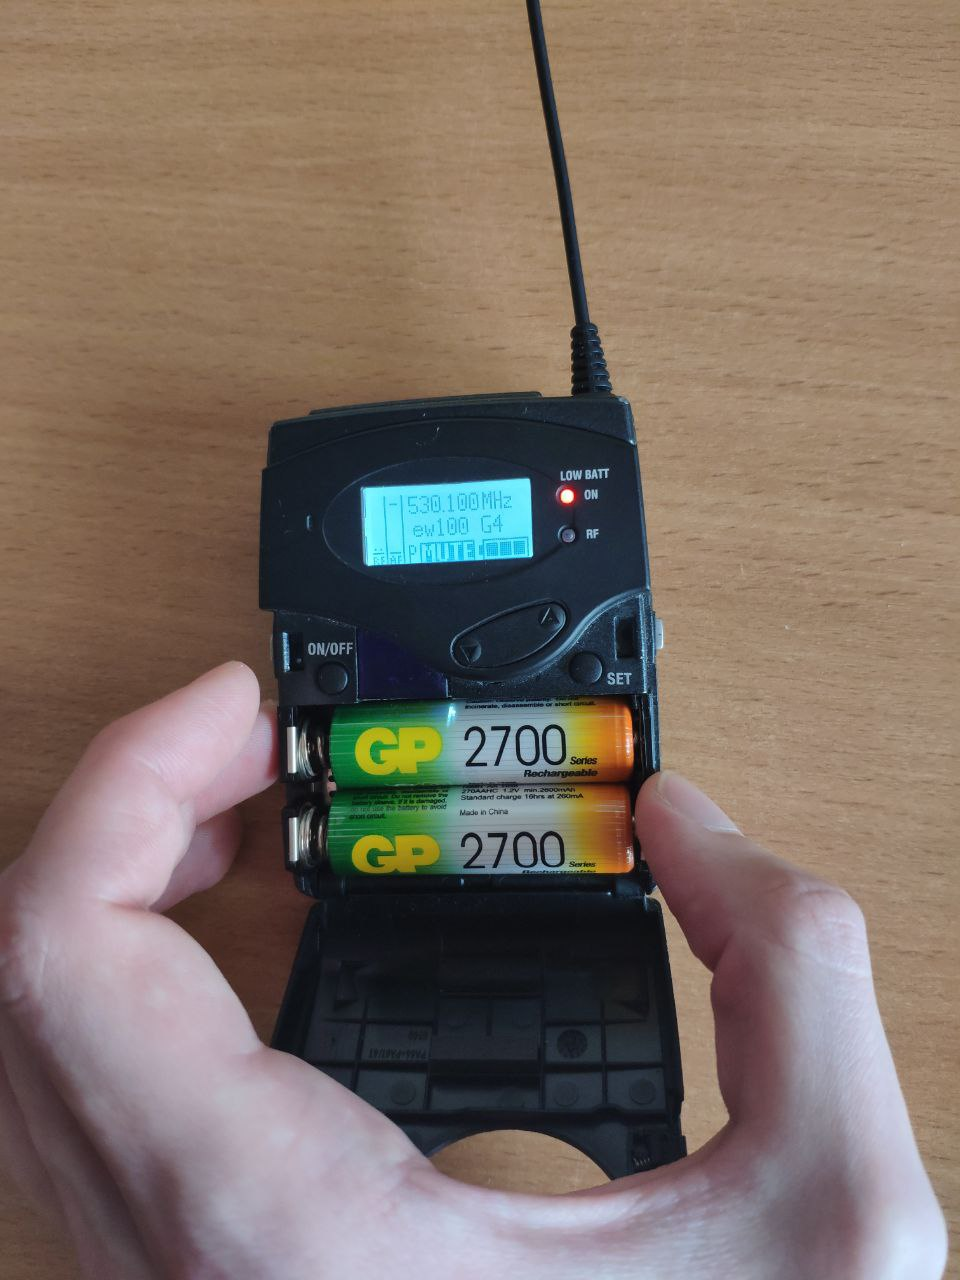
\includegraphics[width=\textwidth]{Images/PortableCamera/micro/step10.2-3-micro-on.jpg}
                \end{minipage}

          \item Подключить \mitem{receiver} к камере.
                \par Один конец переходника \textsf{XLR -- 3.5 mm jack} присоединить к петличке (\textbf{не закручивать туго винт!}), а второй конец --- к камере в разъём \mitem{INPUT1}. Чтобы провод зашёл, его нужно повернуть отверстием вверх. При успешной вставке вы услышите щелчок.

                \begin{minipage}[c]{0.29\textwidth}
                  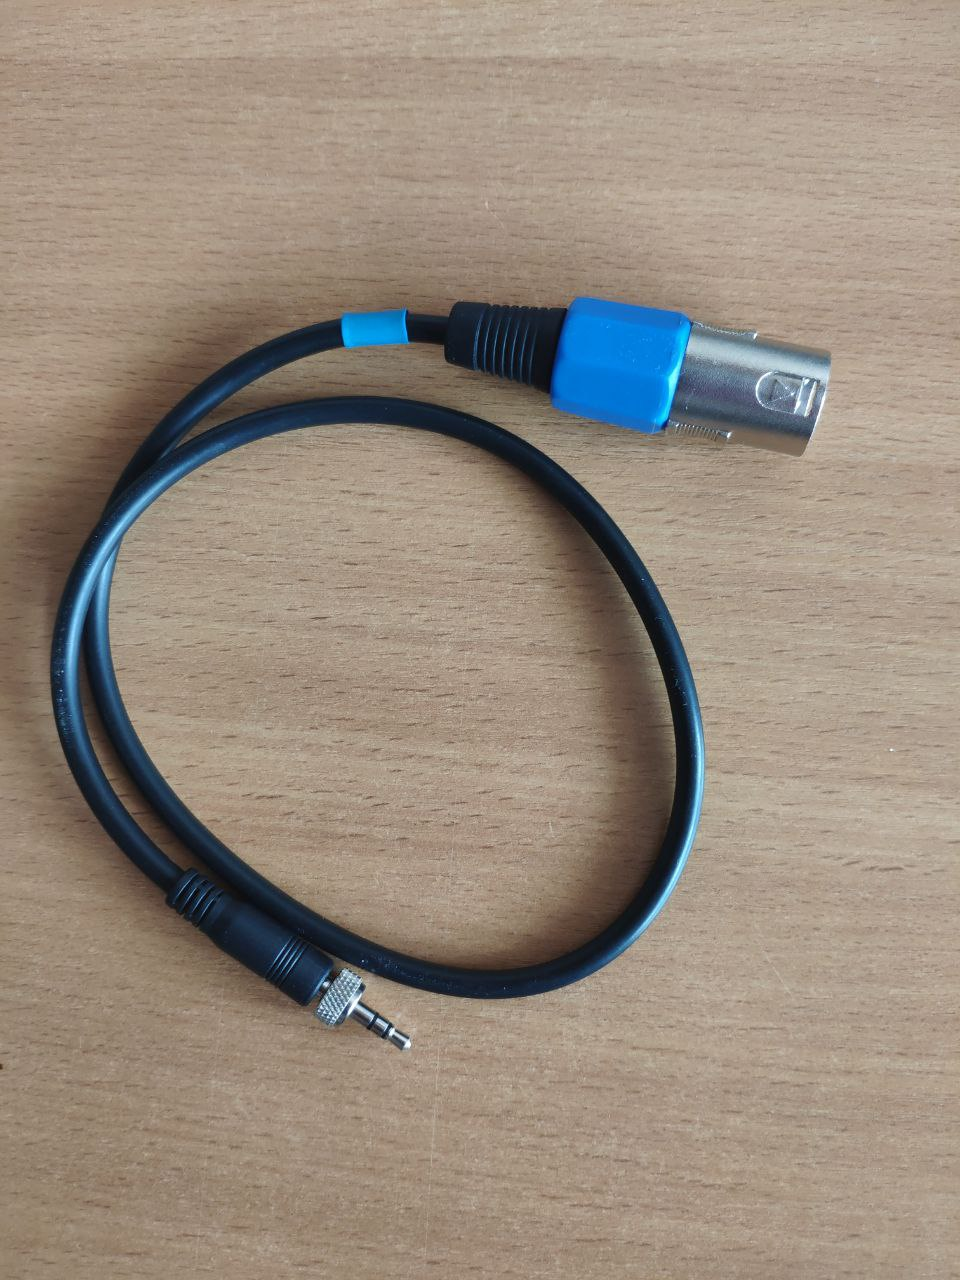
\includegraphics[width=\textwidth]{Images/PortableCamera/micro/step10.3-1-xlr-adapter.jpg}
                \end{minipage}
                \hfill
                \begin{minipage}[c]{0.29\textwidth}
                  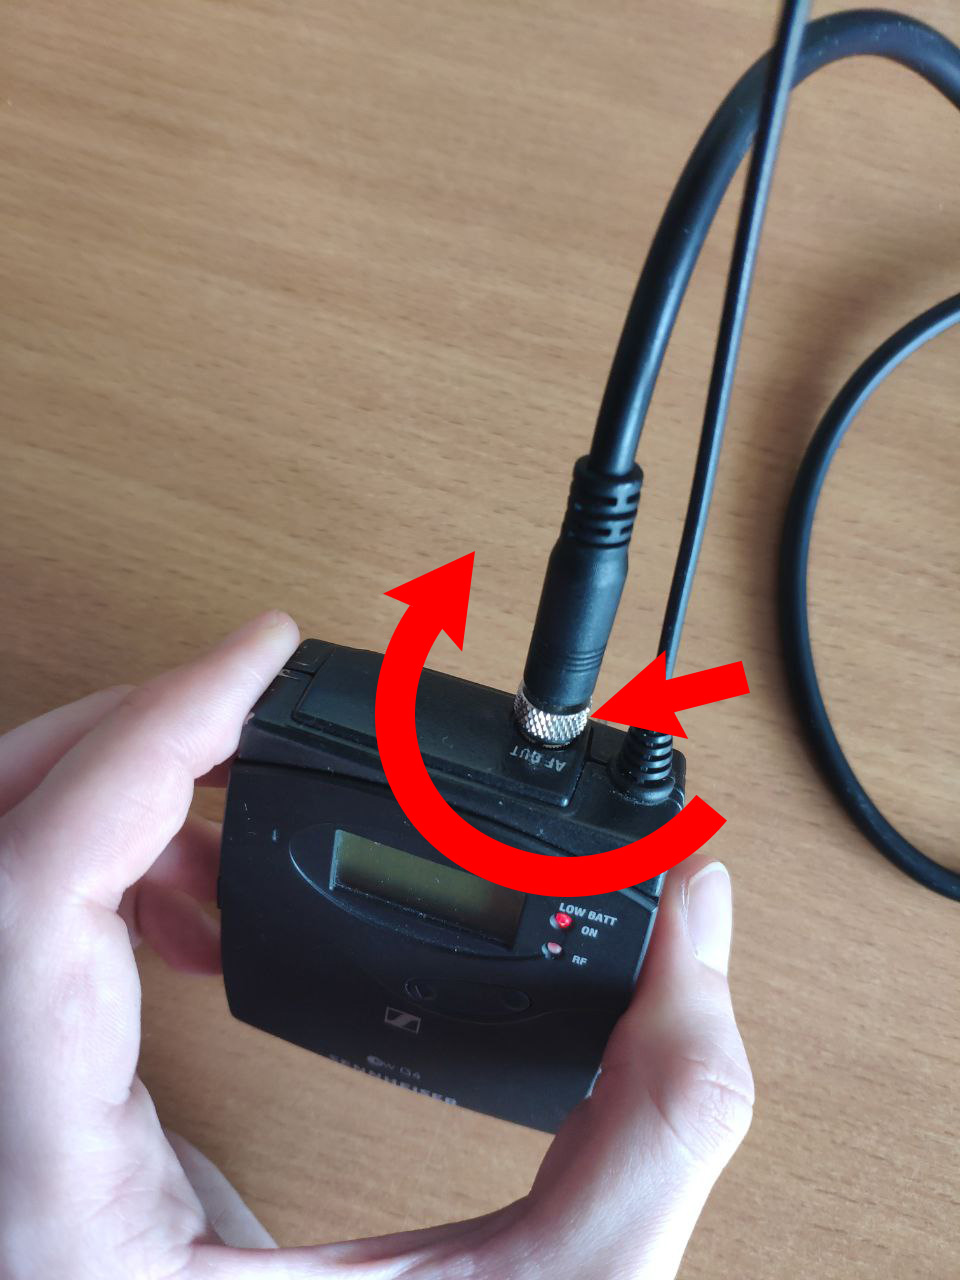
\includegraphics[width=\textwidth]{Images/PortableCamera/micro/step10.3-2-jack-in-micro.jpg}
                \end{minipage}
                \hfill
                \begin{minipage}[c]{0.29\textwidth}
                  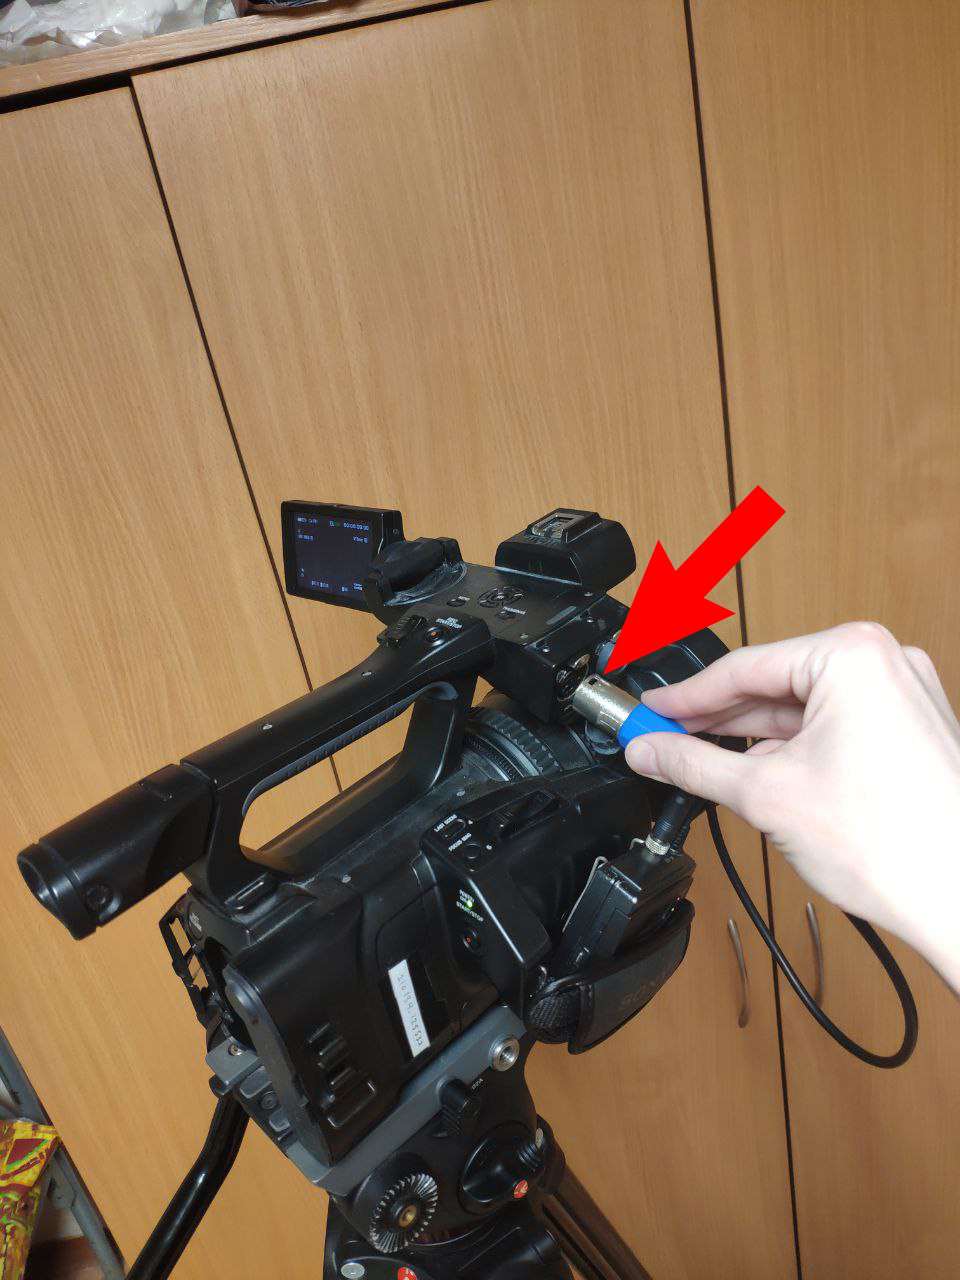
\includegraphics[width=\textwidth]{Images/PortableCamera/micro/step10.3-3-xlr-to-camera.jpg}
                \end{minipage}

          \item Расположить \mitem{receiver} между боковой ручкой и камерой.

                \begin{center}
                  \begin{minipage}[c]{0.45\textwidth}
                    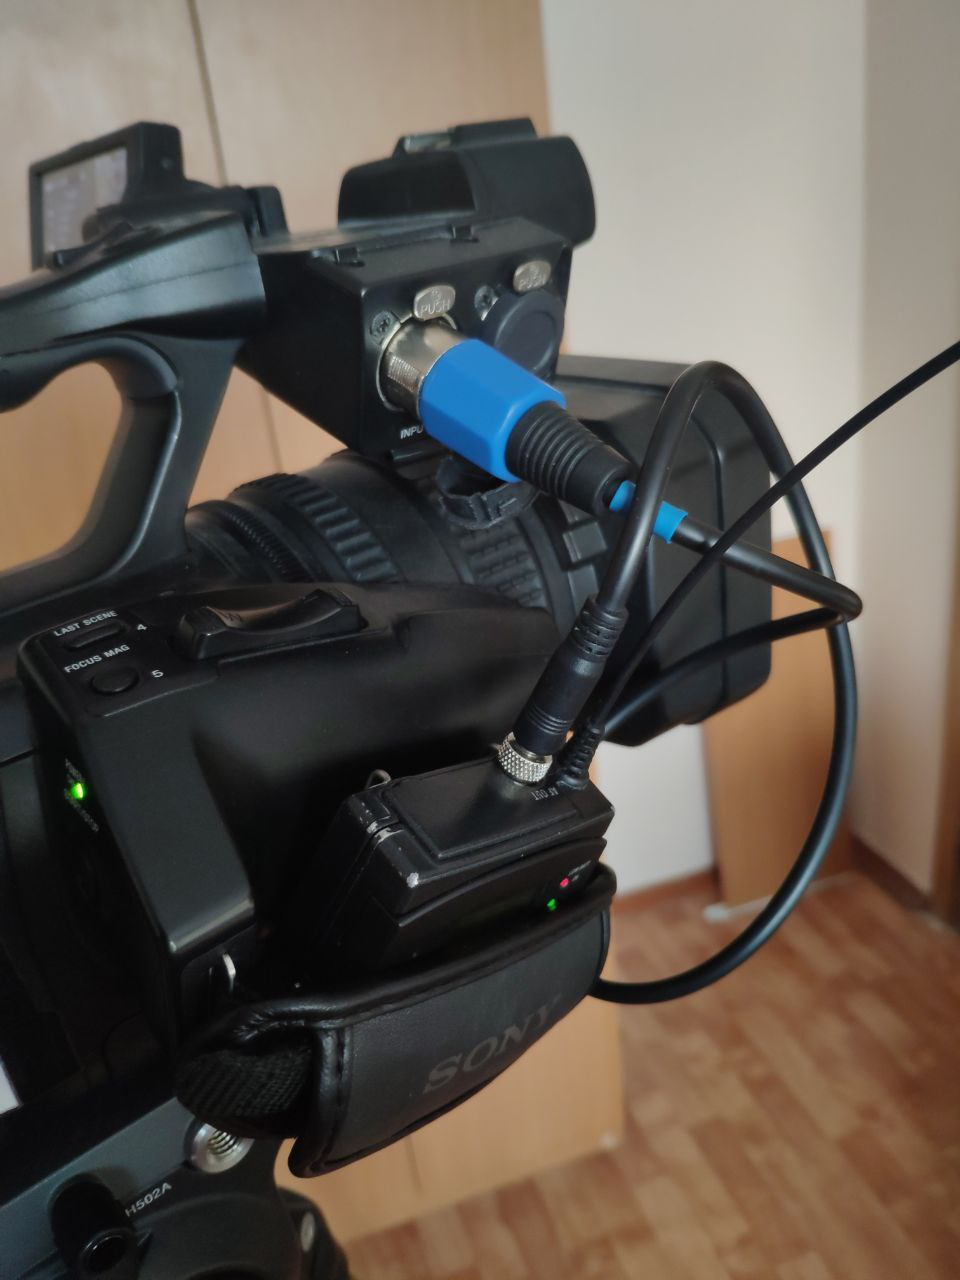
\includegraphics[width=\textwidth]{Images/PortableCamera/micro/step10.4-micro-fixed.jpg}
                  \end{minipage}
                \end{center}

          \item Включить \mitem{transmitter} и прикрепить к нему провод с микрофоном.
                \par Аналогично тому, как делали с \mitem{receiver}.

          \item Проверить, что звук с петлички идёт на камеру.
                \par Для этого нужно поднести микрофон ко рту на расстоянии 1-2 сантиметра и слегка подуть (сделать это бесшумно, чтобы вас не услышал основной микрофон камеры). Если в окошке просмотра ползунок \mitem{CH1} справа снизу зашкаливает тогда и только тогда, когда вы дуете, значит, микрофон работает (на ползунок \mitem{CH2} смотреть нет смысла --- это звук с внутреннего микрофона камеры). Если звука нет, скорее всего на \mitem{transmitter}-е включён режим \mitem{mute} (либо вы забыли включить петлички --- посмотрите, что на их окошках горят символы). На картинке показано положение, в котором должен быть установлен переключатель \mitem{mute}, чтобы был звук.

                \begin{minipage}[c]{0.45\textwidth}
                  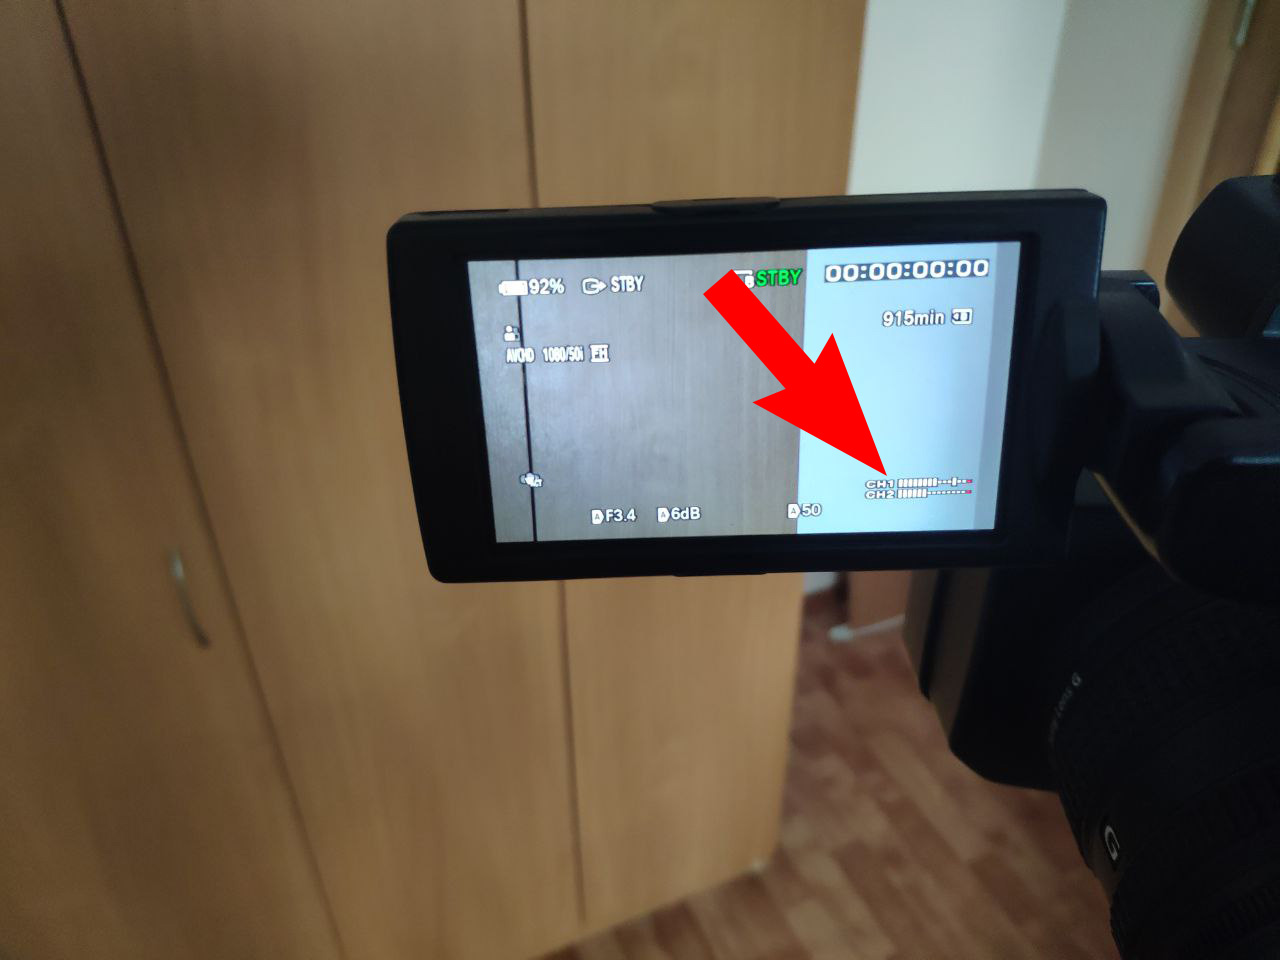
\includegraphics[width=\textwidth]{Images/PortableCamera/micro/step10.6-1-sound-view.jpg}
                \end{minipage}
                \hfill
                \begin{minipage}[c]{0.38\textwidth}
                  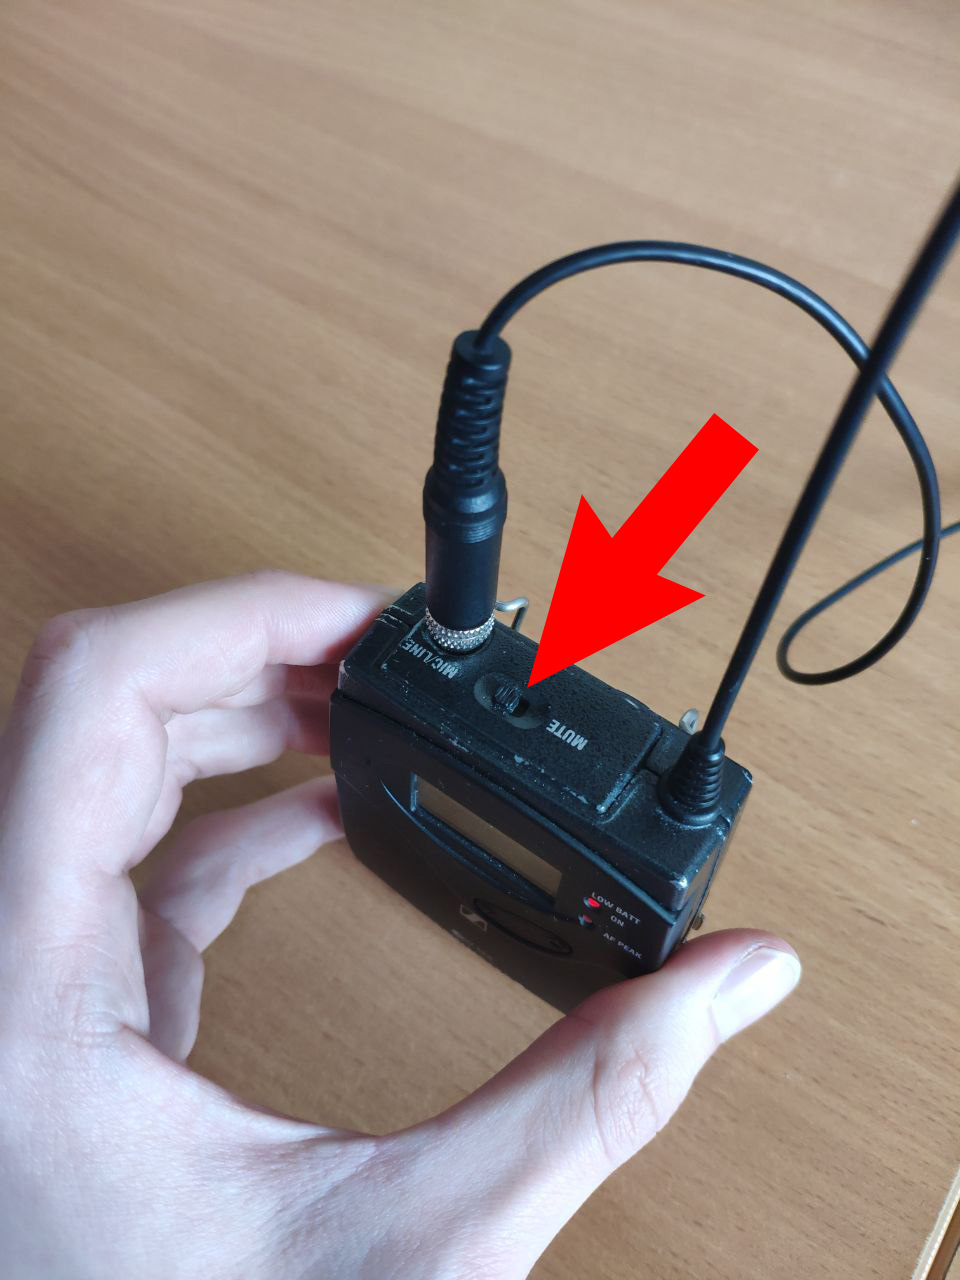
\includegraphics[width=\textwidth]{Images/PortableCamera/micro/step10.6-2-mute.jpg}
                \end{minipage}

                Если звука всё ещё нет, то посмотреть, что положение переключателей на камере соответствует картинке.

                \begin{center}
                  \begin{minipage}[c]{0.55\textwidth}
                    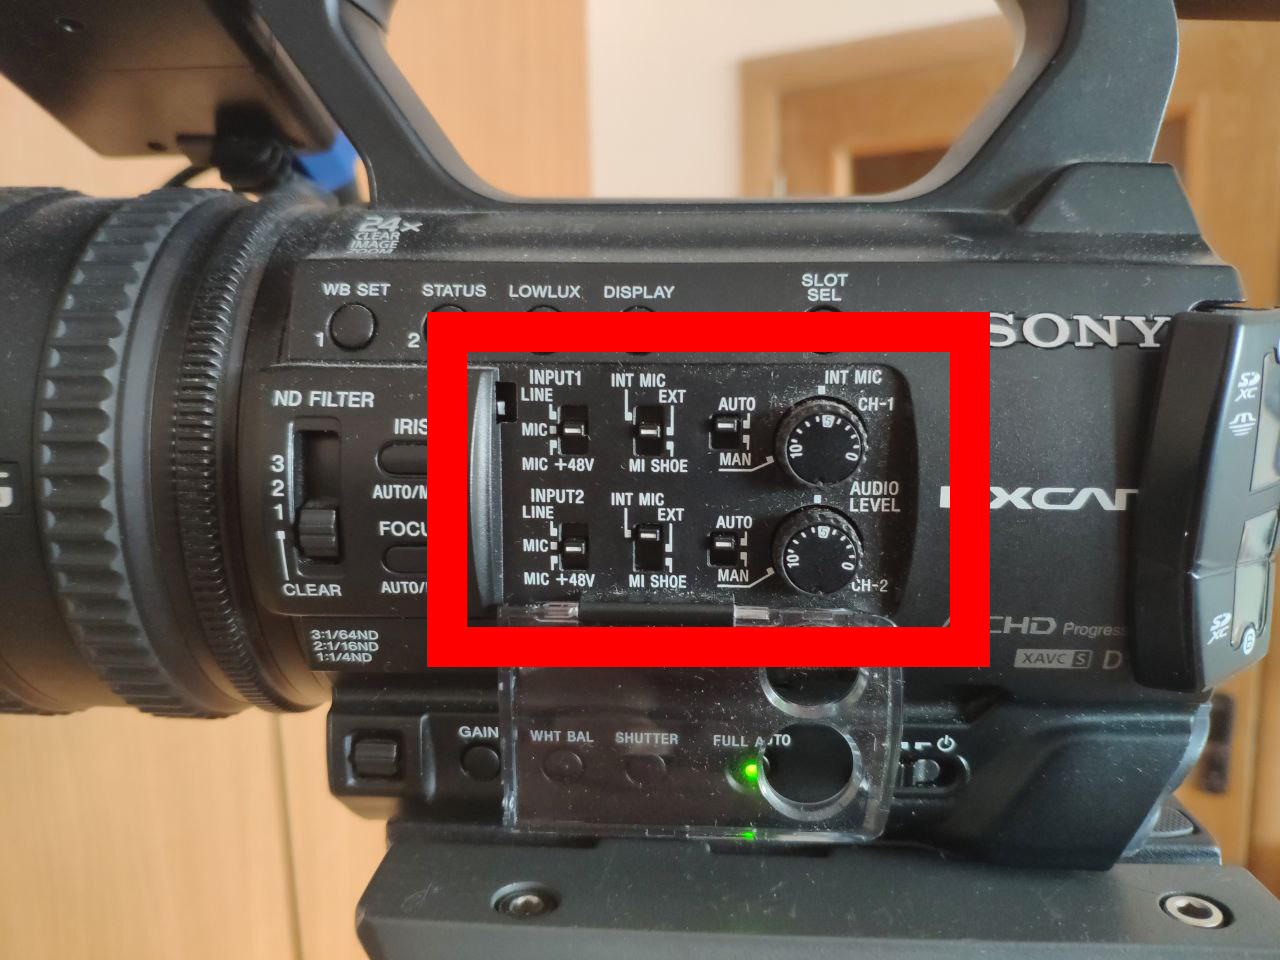
\includegraphics[width=\textwidth]{Images/PortableCamera/micro/step10.6-3-sound-settings.jpg}
                  \end{minipage}
                \end{center}

          \item Отдать transmitter лектору и начать запись, нажав на любую из красных кнопок (они эквивалентны).
                \par Если запись началась, в окошке просмотра появится красный круг.

                \begin{center}
                  \begin{minipage}[c]{0.45\textwidth}
                    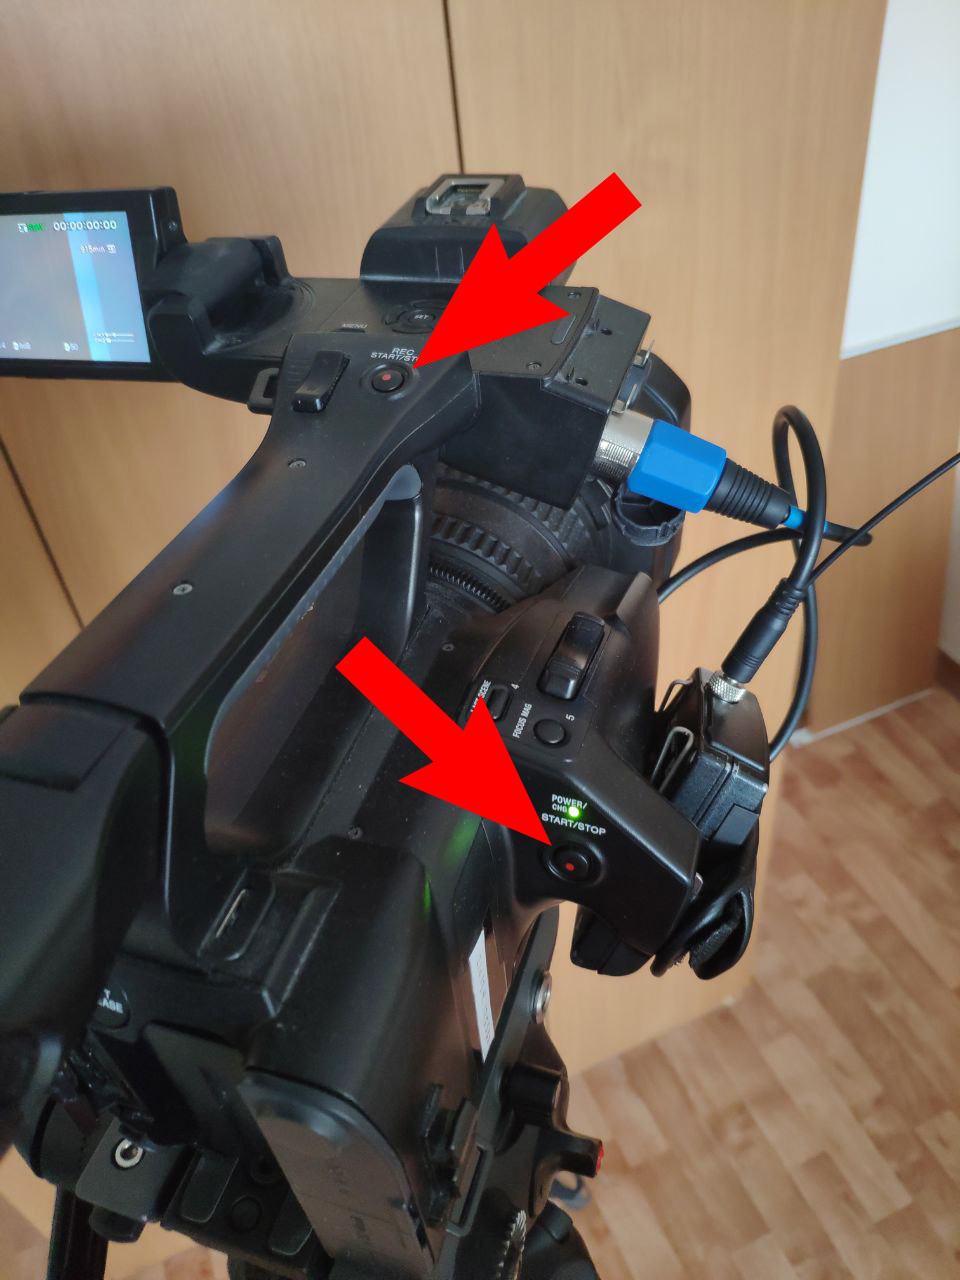
\includegraphics[width=\textwidth]{Images/PortableCamera/recording/step10.7-start-recording.jpg}
                  \end{minipage}
                \end{center}

        \end{enumerate}
\end{enumerate}

%%%%%%%%%%%%%%%%%%%%%%%%%%%%%%%%%%%%%%%%%%%%%%%%%%%%%%%%%
\subsubsection{Как снимать}
%%%%%%%%%%%%%%%%%%%%%%%%%%%%%%%%%%%%%%%%%%%%%%%%%%%%%%%%%

\begin{itemize}
  \item Зум осуществляется либо с помощью колеса, либо по переключателю.

        \begin{minipage}[c]{0.5\textwidth}
          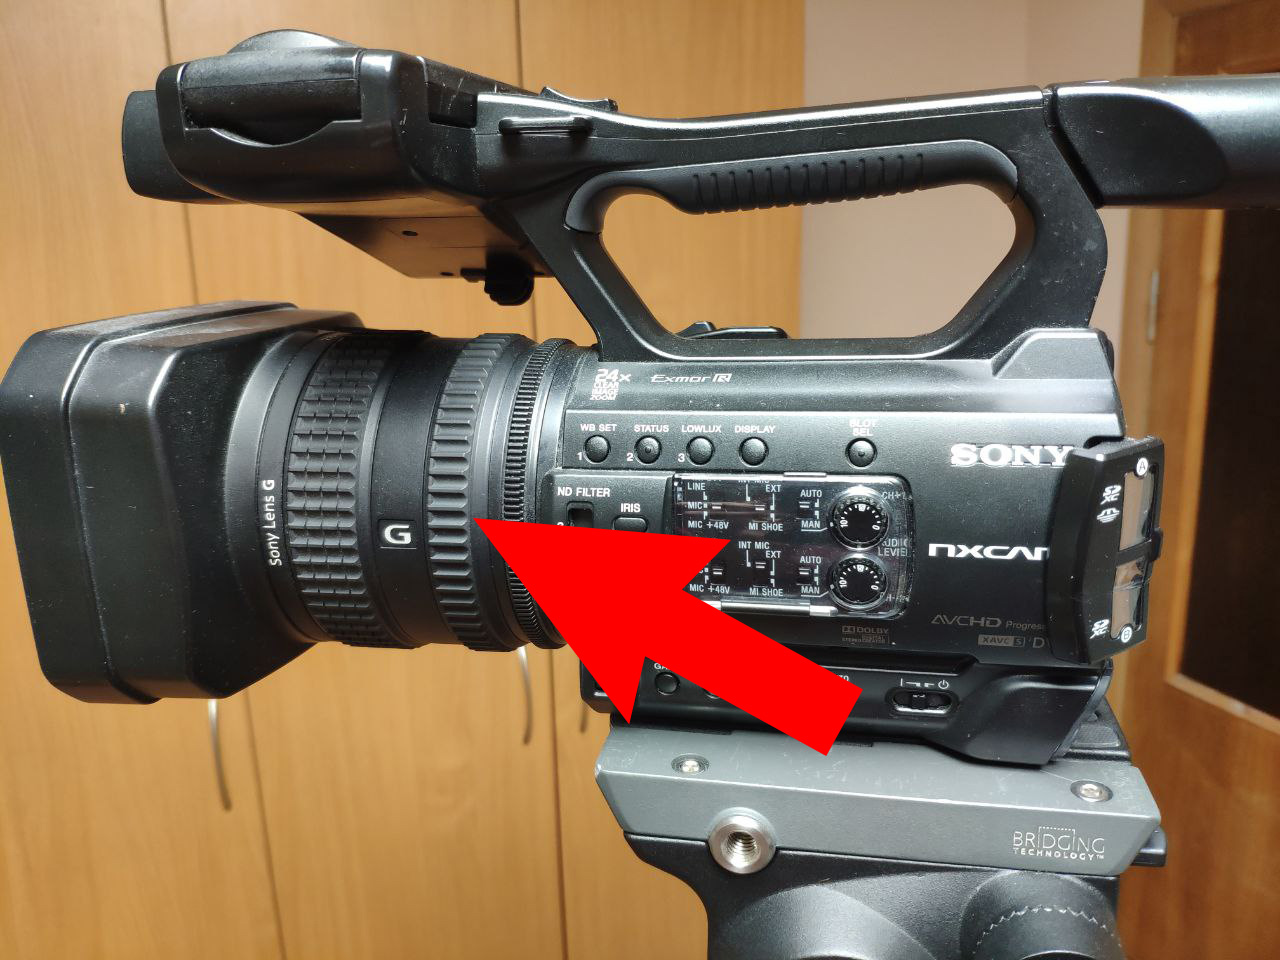
\includegraphics[width=\textwidth]{Images/PortableCamera/recording/zoom-switcher.jpg}
        \end{minipage}
        \hfill
        \begin{minipage}[c]{0.4\textwidth}
          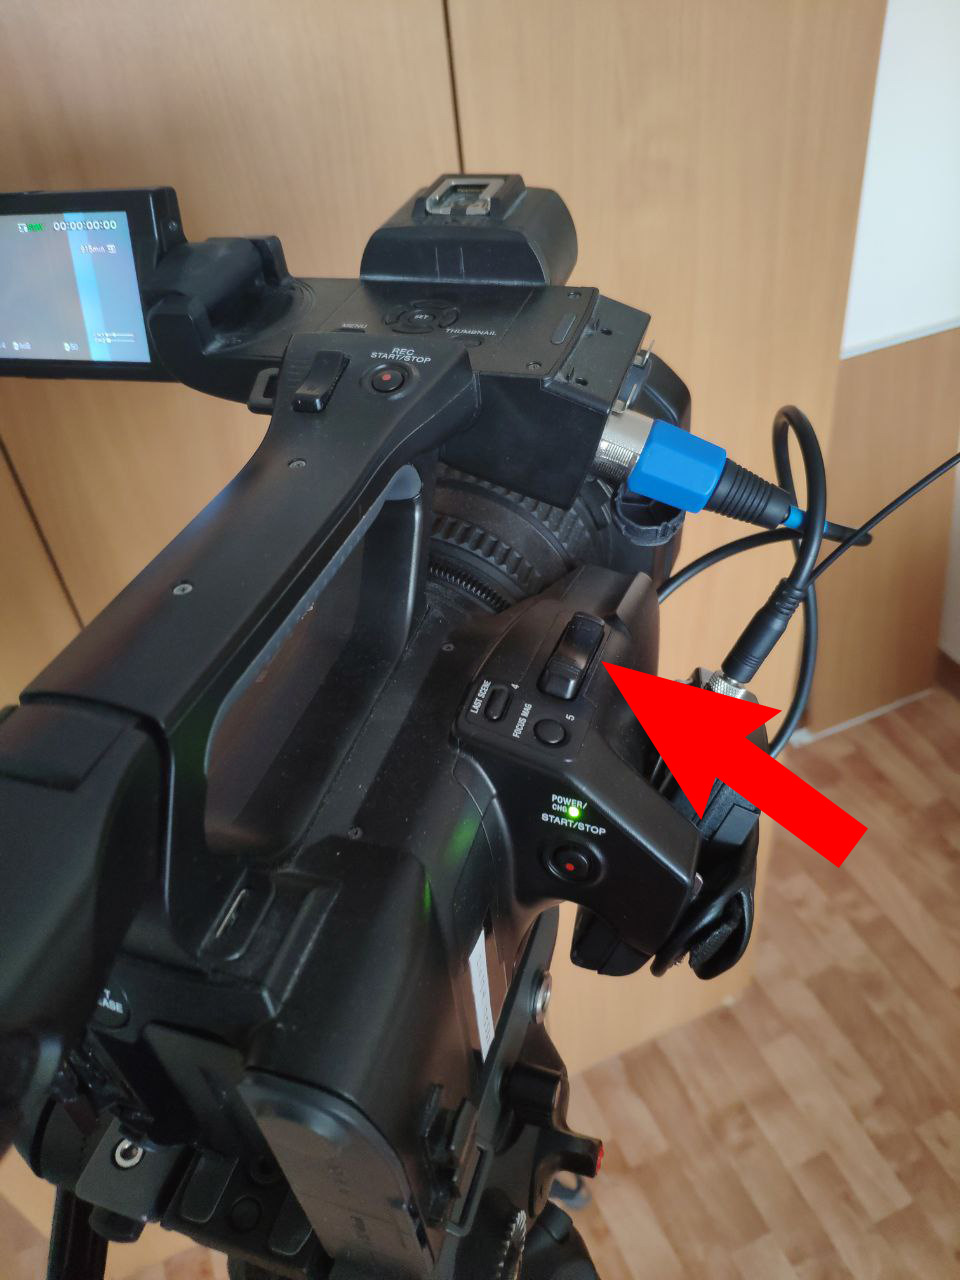
\includegraphics[width=\textwidth]{Images/PortableCamera/recording/zoom-bottom.jpg}
        \end{minipage}

  \item Во время съёмки поглядвайте периодически на дорожку со звуком \mitem{CH1}. Если вы видите, что она расположена в положении 0 и не двигается (либо двигается очень слабо) --- остановите лектора и выясните, что произошло. Возможные причины:
        \begin{itemize}
          \item \textbf{Сели аккумы}. Поменяйте их на запасные (они находятся в нижнем кармане рюкзака). Разряженные аккумы положите в карман рюкзака, где лежат провода от петличек.

          \item \textbf{С лектора упал петличный микрофон}. Проверьте, что лектор правильно закрепляет клипсу.
                \begin{enumerate}
                  \item Клипсу лучше всего прикреплять за разрезы одежды, воротники и прочее, чтобы она не выскальзывала.
                  \item Проверьте, что провод с микрофоном не натянут (иногда лекторы стараются засунуть провод в карман, чтобы <<лишнее не торчало>>)
                \end{enumerate}
        \end{itemize}
\end{itemize}

%%%%%%%%%%%%%%%%%%%%%%%%%%%%%%%%%%%%%%%%%%%%%%%%%%%%%%%%%
\subsubsection{Как разбирать комплект}
%%%%%%%%%%%%%%%%%%%%%%%%%%%%%%%%%%%%%%%%%%%%%%%%%%%%%%%%%

\begin{enumerate}
  \item Первым делом нужно \textbf{забрать \mitem{transmitter} у лектора}.
        \par Некоторые лекторы забывают про его существование и уходят прямо с ним :) .

  \item Выключить \mitem{transmitter} и положить провод в верхний карман рюкзака.
        \par \textbf{Не забывайте откручивать винт} перед тем, как достать провод из петлички. Для выключения зажать кнопку \mitem{ON/OFF} на 2-3 секунды.

  \item Отключить \mitem{receiver} и положить провод в верхний карман рюкзака.
        \par Для того чтобы отключить провод от камеры, нужно зажать язычок \mitem{push} и вытянуть провод. В остальном действия аналогичны сборке.

        \begin{center}
          \begin{minipage}[c]{0.45\textwidth}
            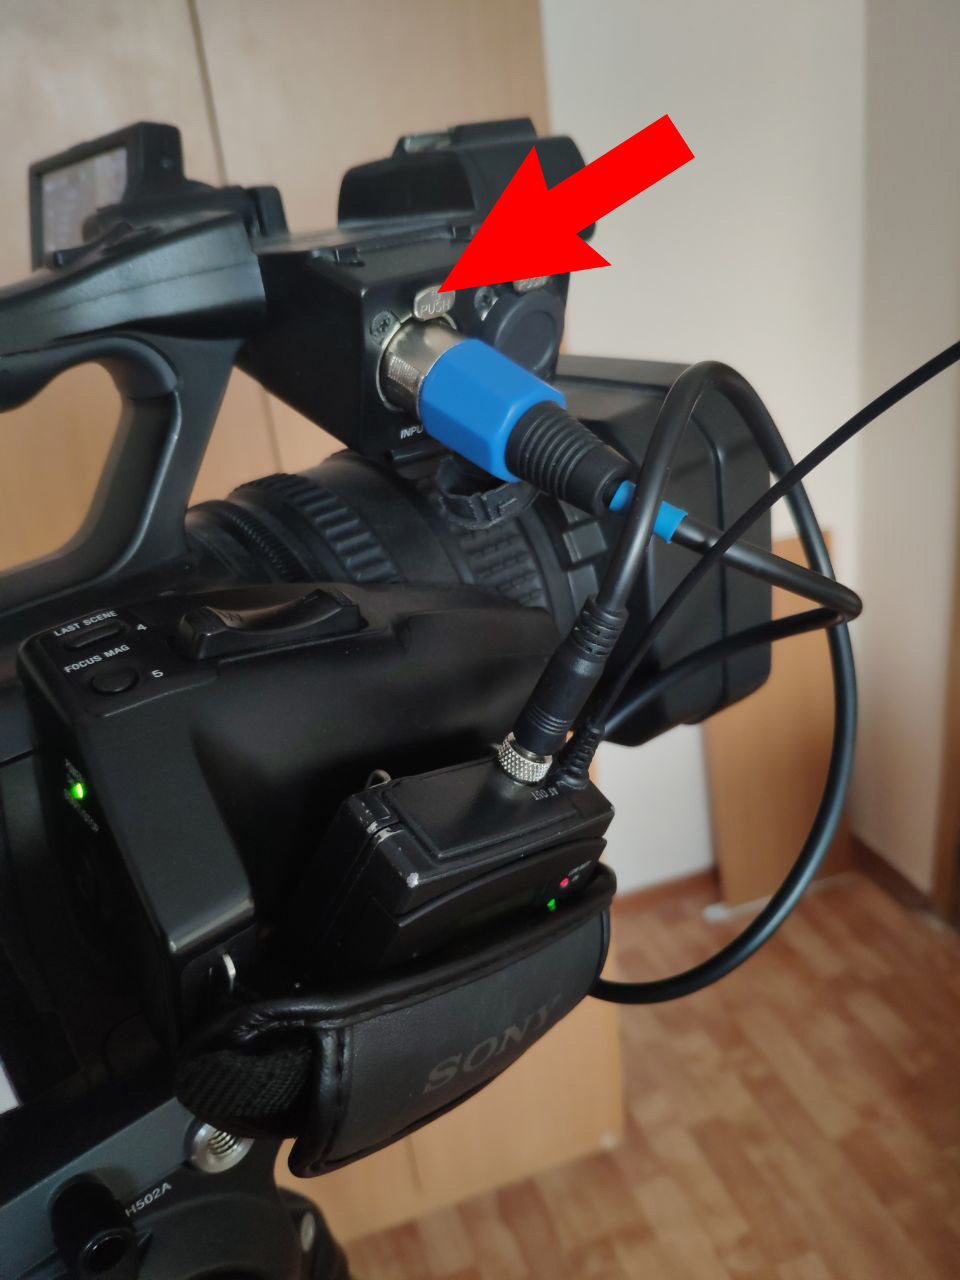
\includegraphics[width=\textwidth]{Images/PortableCamera/recording/pull-out-xlr.jpg}
          \end{minipage}
        \end{center}

  \item Положить петлички в рюкзак \textbf{антеннами вниз и вперёд}.
        \par Может показаться, что антенна одной из петличек при таком подходе не влезает. Однако её просто нужно расположить справа от верхнего кармана рюкзака. Верхний карман приклеплён на липучках, поэтому там будет место. \hyperref[fig:camera-in-bag]{Картинка}.

  \item Выключить камеру и \textbf{надеть на объектив крышку}.
        \par Для выключения нажать на кнопку включения с левой стороны камеры.

  \item Снять камеру со штатива.
        \par Для этого открутить фиксатор 1, зажать чёрную кнопку 2 и вытянуть камеру на себя, держа её за верхнюю ручку. \hyperref[fig:retainer]{Картинка}.

  \item Положить камеру в рюкзак объективом вперёд, кнопками --- вниз.

        \begin{center}
          \begin{minipage}[c]{0.45\textwidth}\label{fig:camera-in-bag}
            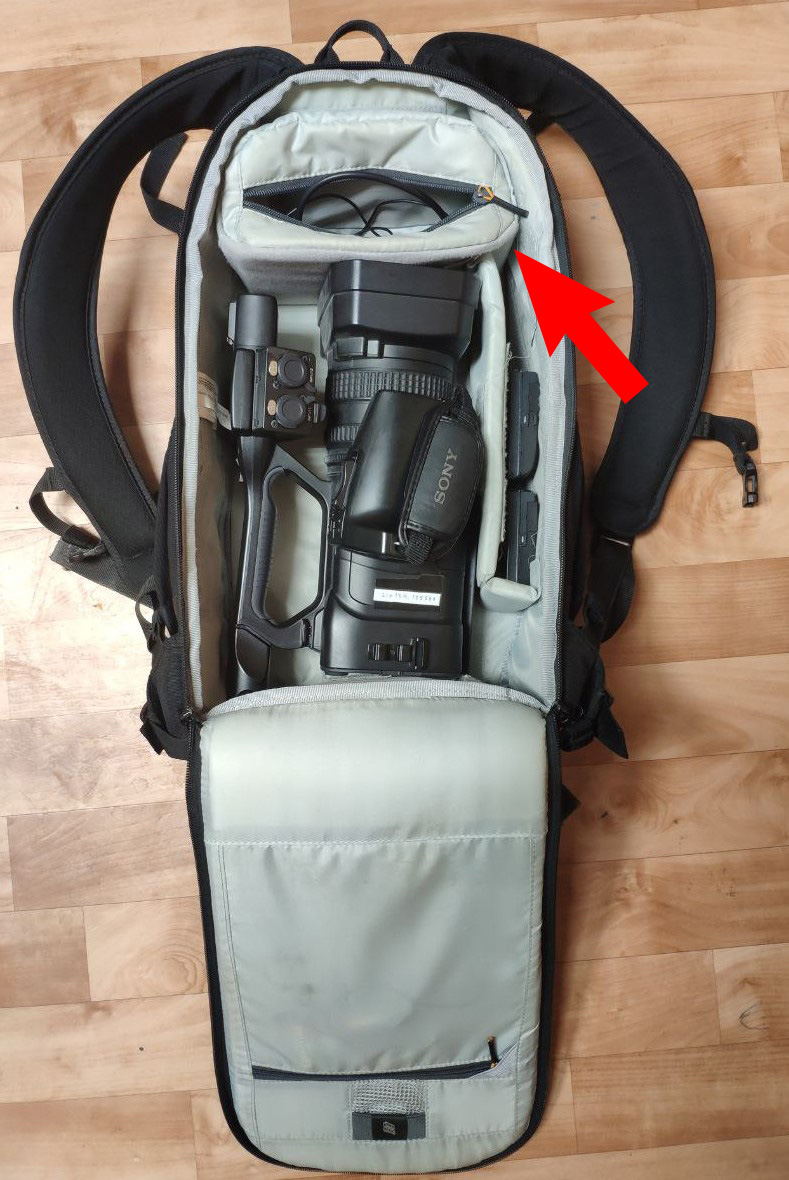
\includegraphics[width=\textwidth]{Images/PortableCamera/recording/camera-in-bag.jpg}
          \end{minipage}
        \end{center}

  \item Сложить штатив:
        \begin{enumerate}
          \item Собрать ноги вместе (потянуть среднюю растяжку вверх).

                \begin{center}
                  \begin{minipage}[c]{0.45\textwidth}
                    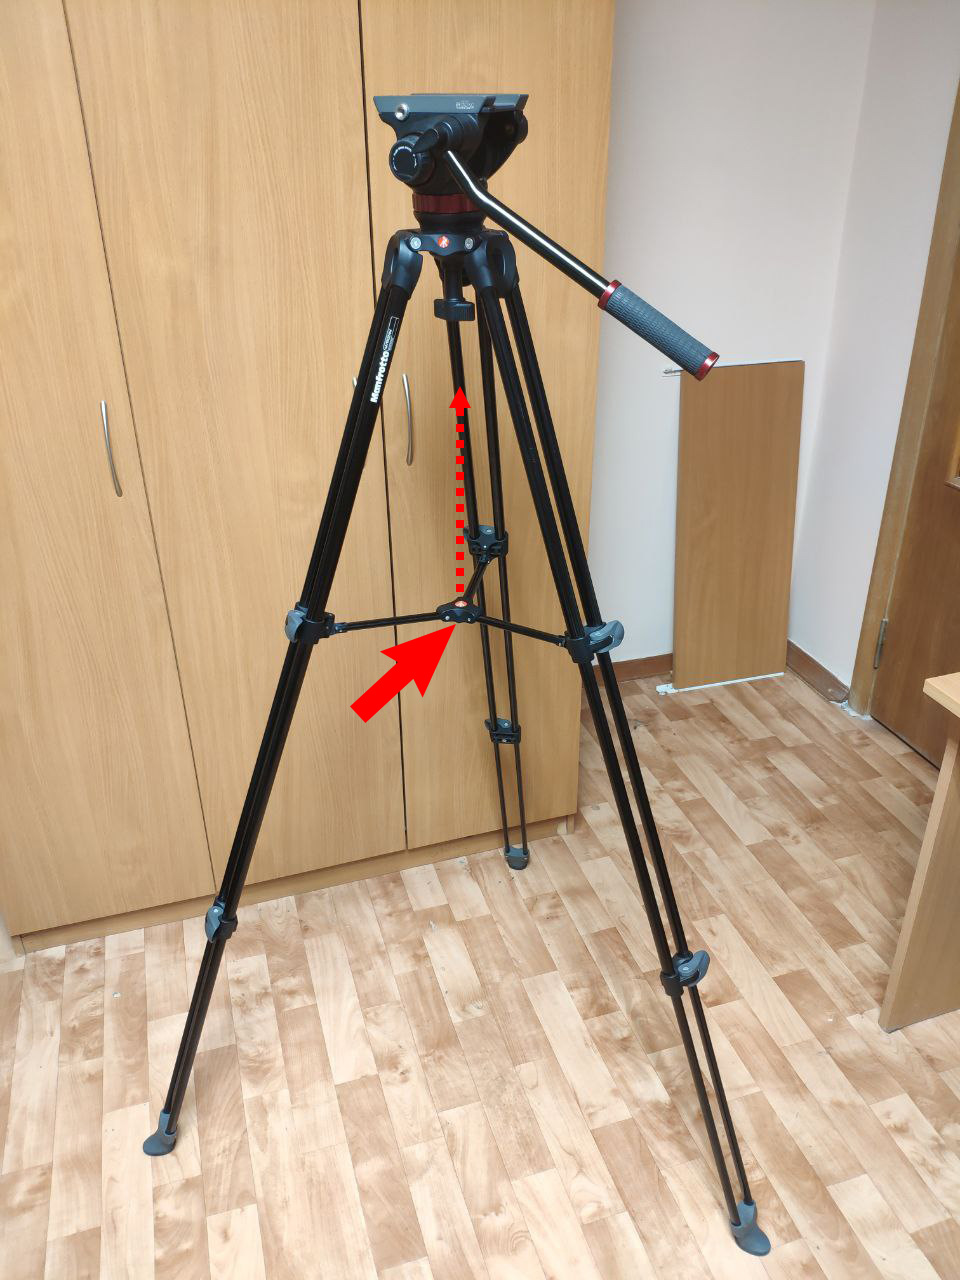
\includegraphics[width=\textwidth]{Images/PortableCamera/tripod/stretch-legs-apart.jpg}
                  \end{minipage}
                \end{center}

          \item Открепить серые зажимы и перевести штатив в положение на картинке, закрепить зажимы. \textbf{Только после этого} открутить ручку, прижать её к ногам и прикрутить обратно.

                \begin{minipage}[c]{0.4\textwidth}
                  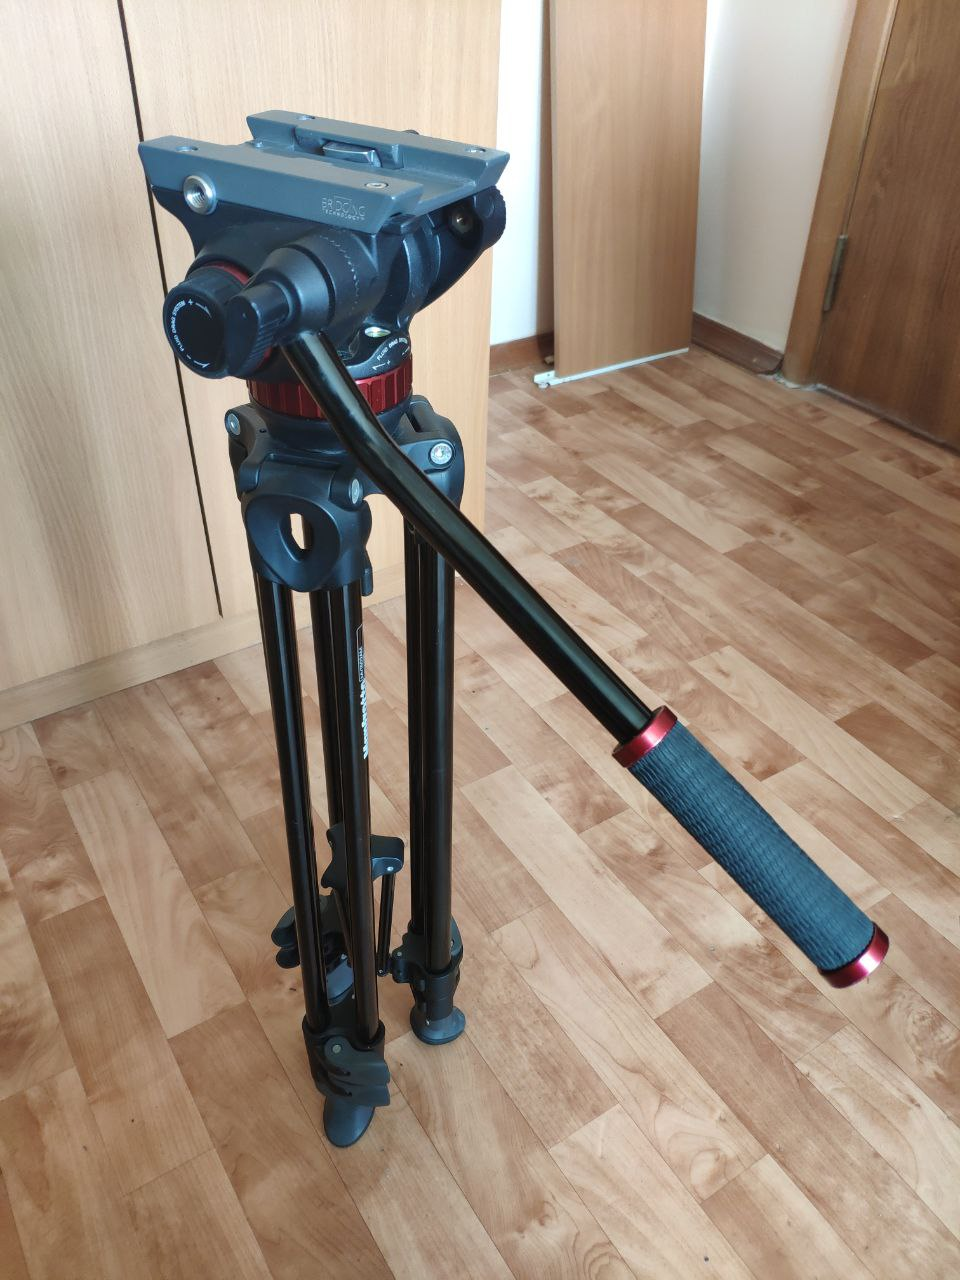
\includegraphics[width=\textwidth]{Images/PortableCamera/tripod/fold-handle-on.jpg}
                \end{minipage}
                \hfill
                \begin{minipage}[c]{0.4\textwidth}
                  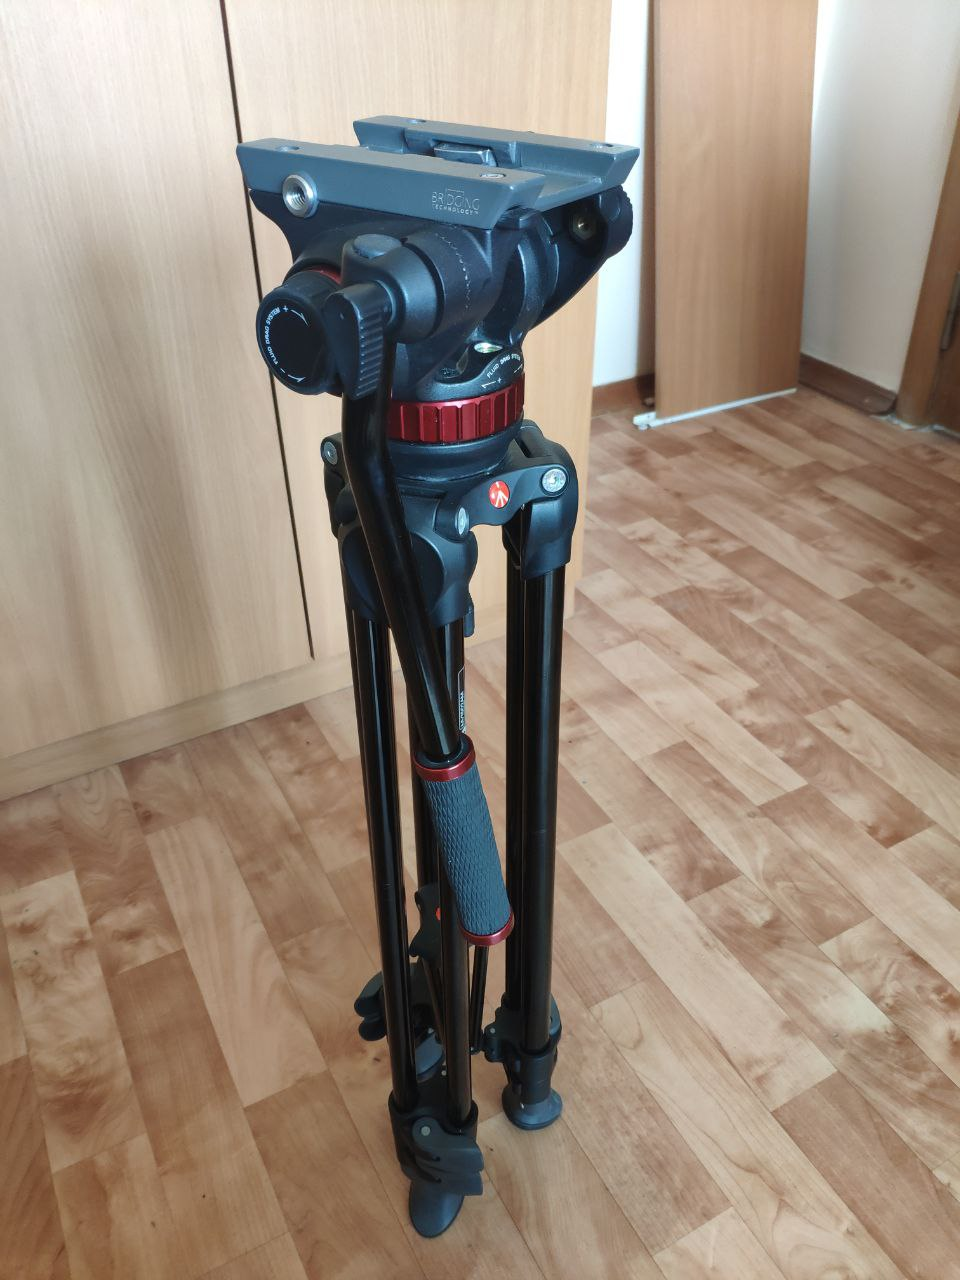
\includegraphics[width=\textwidth]{Images/PortableCamera/tripod/fold-habdle-off.jpg}
                \end{minipage}

          \item Положить штатив в чехол, \textbf{закрепив его липучкой}.
        \end{enumerate}
\end{enumerate}

% %%%%%%%%%%%%%%%%%%%%%%%%%%%%%%%%%%%%%%%%%%%%%%%%%%%%%%%%%
% \subsubsection{Как менять аккумулятор у камеры}
% %%%%%%%%%%%%%%%%%%%%%%%%%%%%%%%%%%%%%%%%%%%%%%%%%%%%%%%%%

\partodo{Секция: как менять аккумулятор у камеры}

